% arara: xelatex: { shell: yes }
% narara: makeglossaries
% narara: biber
% narara: xelatex: { shell: yes }
% narara: xelatex: { shell: yes }
\documentclass[thesis=B,czech,hidelinks]{src/FITthesisXE}

\usepackage{ graphicx }
\usepackage{ dirtree }
\usepackage{ longtable } 

\bibliography{library.bib}

\makeglossaries
\newacronym{VR}{VR}{virtuální realita}
\newacronym{API}{API}{application programming interface}
\newacronym{POC}{POC}{proof of concept}
\newacronym{OLED}{OLED}{virtuální}
\newacronym{OSVR}{OSVR}{virtuální}
\newacronym{MSDN}{MSND}{virtuální}
\newacronym{SDK}{SDK}{virtuální}
\newacronym{WPF}{WPF}{Windows Presentation Foundation}
\glsaddall

%%%

\acknowledgements{Děkuji svému vedoucímu práce, panu Jiřímu Chludilovi, za jeho pomoc, vstřícný přístup a věcné rady při vedení této práce.

Děkuji také herně \emph{Virtualnirealita.cz} za zapůjčení vybavení a poskytnutí užitečných dat o zákaznících pro analýzu.

Chtěl bych poděkovat Janě Kubíčkové a Jarmile Hlaváčové za zpětnou vazbu k textu závěrečné práce.

Dále bych chtěl poděkovat Jakubovi Jirůtkovi za svolení použít a upravit jeho technické řešení sazby práce a za jeho účast při testování aplikace.

Poděkování patří i Tomášovi Havlíkovi za jeho účast na testování a za jeho ...}

\abstractCS{Tato práce se zabývá zefektivněním procesu seznámení uživatelů
s~virtuální realitou v~prostředí nově vzniklých heren virtuální reality.
Za cíl si klade předat informace, které sděluje obsluha zákazníkům,
rychlou a~zároveň plnohodnotnou formou prostřednictvím aplikace spuštěné
přímo ve virtuální realitě. Jelikož se tématicky práce týká relativně
nového trendu --- virtuální reality, pracuje s~moderní, atraktivní a
v~současnosti nepříliš běžnou hardwarovou i softwarovou výbavou. Výsledkem
práce je analýza, návrh aplikace a~její realizace, společně s~testováním
v~reálném prostředí herny virtuální reality.
}
\abstractEN{The thesis deals with process of familiarizing users to the virtual
reality more effective. The objective is to exchange the important
information, that are told by the arcade crew to their customers, the
quicker but complete way, though an virtual reality application. Thanks
to the virtual reality topic, this work approaches an attractive, modern
and unusual hardware devices and software libraries and resources. The
result of this thesis is analysis, application design and realization of
designed application, together with testing in a real environment of
virtual reality arcade.
}

\department{Katedra softwarového inženýrství}
\title{Výuková aplikace pro systémy virtuální reality}

\authorGN{Marián}
\authorFN{Hlaváč}
\authorWithDegrees{Marián Hlaváč}
\supervisor{Ing. Jiří Chludil}

\keywordsCS{výuková aplikace, virtuální realita, implementace, výuka, herní průmysl, htc vive}
\keywordsEN{education application, virtual reality, implementation, education, game industry, htc vive}

\placeForDeclarationOfAuthenticity{V~Praze}
\declarationOfAuthenticityOption{1} %volba Prohlášení (číslo 1-6)

% \website{http://site.example/thesis}

\begin{document}

\begin{introduction}
\label{introduction}
	Virtuální realita (často zkracována na VR) je bezesporu novým trendem v
oblasti informačních technologií. Protože je tato technologie běžným
lidem méně dostupná, vznikly ve větších městech nové podniky, které
zprostředkovávají zážitky ve virtuální realitě za zlomek ceny celého
systému bez nutnosti znalosti systémů virtuální reality, zajištění
dostatečného výpočetního výkonu, výběru a nákupu aplikací pro virtuální
realitu kompatibilní s konkrétním systémem a konfigurace virtuální
reality. Tyto podniky se označují jako \emph{herny virtuální reality}. \autocite{herny}

Návštěvníci pak kladou na takové podniky jisté požadavky, na které
systémy virtuální reality nejsou v současné době plně připraveny.
Uživatelské rozhraní softwaru je navrženo spíše na jednoho dlouhodobého
uživatele, který měl prostor systému porozumět, což je nevhodné v
prostředí, kde se uživatel s virtuální realitou setkává poprvé a v
omezeném čase, po který mu byl systém zapůjčen.

\section{Co je virtuální
realita}\label{co-je-virtuuxe1lnuxed-realita}

Pojem virtuální realita označuje technologii prezentace prostředí pomocí
replikace lidských smyslů tak, aby simulovala přítomnost uživatele v
takovém prostředí. Často se virtuální realitou označuje i samotné
prostředí. Technologie tak vytváří iluzi reálného alternativního světa. \autocite{ovr}

Konkrétní definici virtuální reality v angličtině: ``a realistic and
immersive simulation of a three-dimensional 360-degree environment,
created using interactive software and hardware, and experienced or
controlled by movement of the body'' \autocite{vrdef} lze přeložit jako ``realistická a
pohlcující simulace trojrozměrného 360 stupňového prostředí tvořeného
pomocí interaktivního softwaru a hardwaru ovládaného pohybem lidského
těla''.

Uživatel virtuální reality se může v prostředí typicky rozhlížet,
procházet se (v různě omezené míře) a interagovat s vyzobrazenými
objekty. \autocite{vrdef2} Virtuální realita nalézá uplatnění v průmyslu, lékařství,
sportu, armádě a především i v zábavním průmyslu. \autocite{vrusage}

Počátky virtuální reality sahají až do 50. let 18. století, kdy se
experimentovalo s různými stereoskopickými displeji a zprostředkováním
jevů ostatních lidských smyslů. Jako nejranější známý příklad virtuální
reality je přístroj zvaný \emph{Sensorama}, který byl schopen zobrazovat
trojrozměrné stereoskopické obrázky, přehrávat zvuk prostředí a
vypouštět aromatické látky pro pohlcující zážitek. \autocite{oldvr}

Na počátku 20. století se objevily další příklady pohlcujících zážitků
virtuální reality. Za zmínku stojí projekční místnost \emph{The Cave},
mezi koncové uživatele nikdy nerozšířený \emph{Sega VR Headset}, či
stejně nepříliš úspěšný \emph{Virtual Boy} od společnosti
\emph{Nintendo}.

\begin{figure}[h!]
\centering
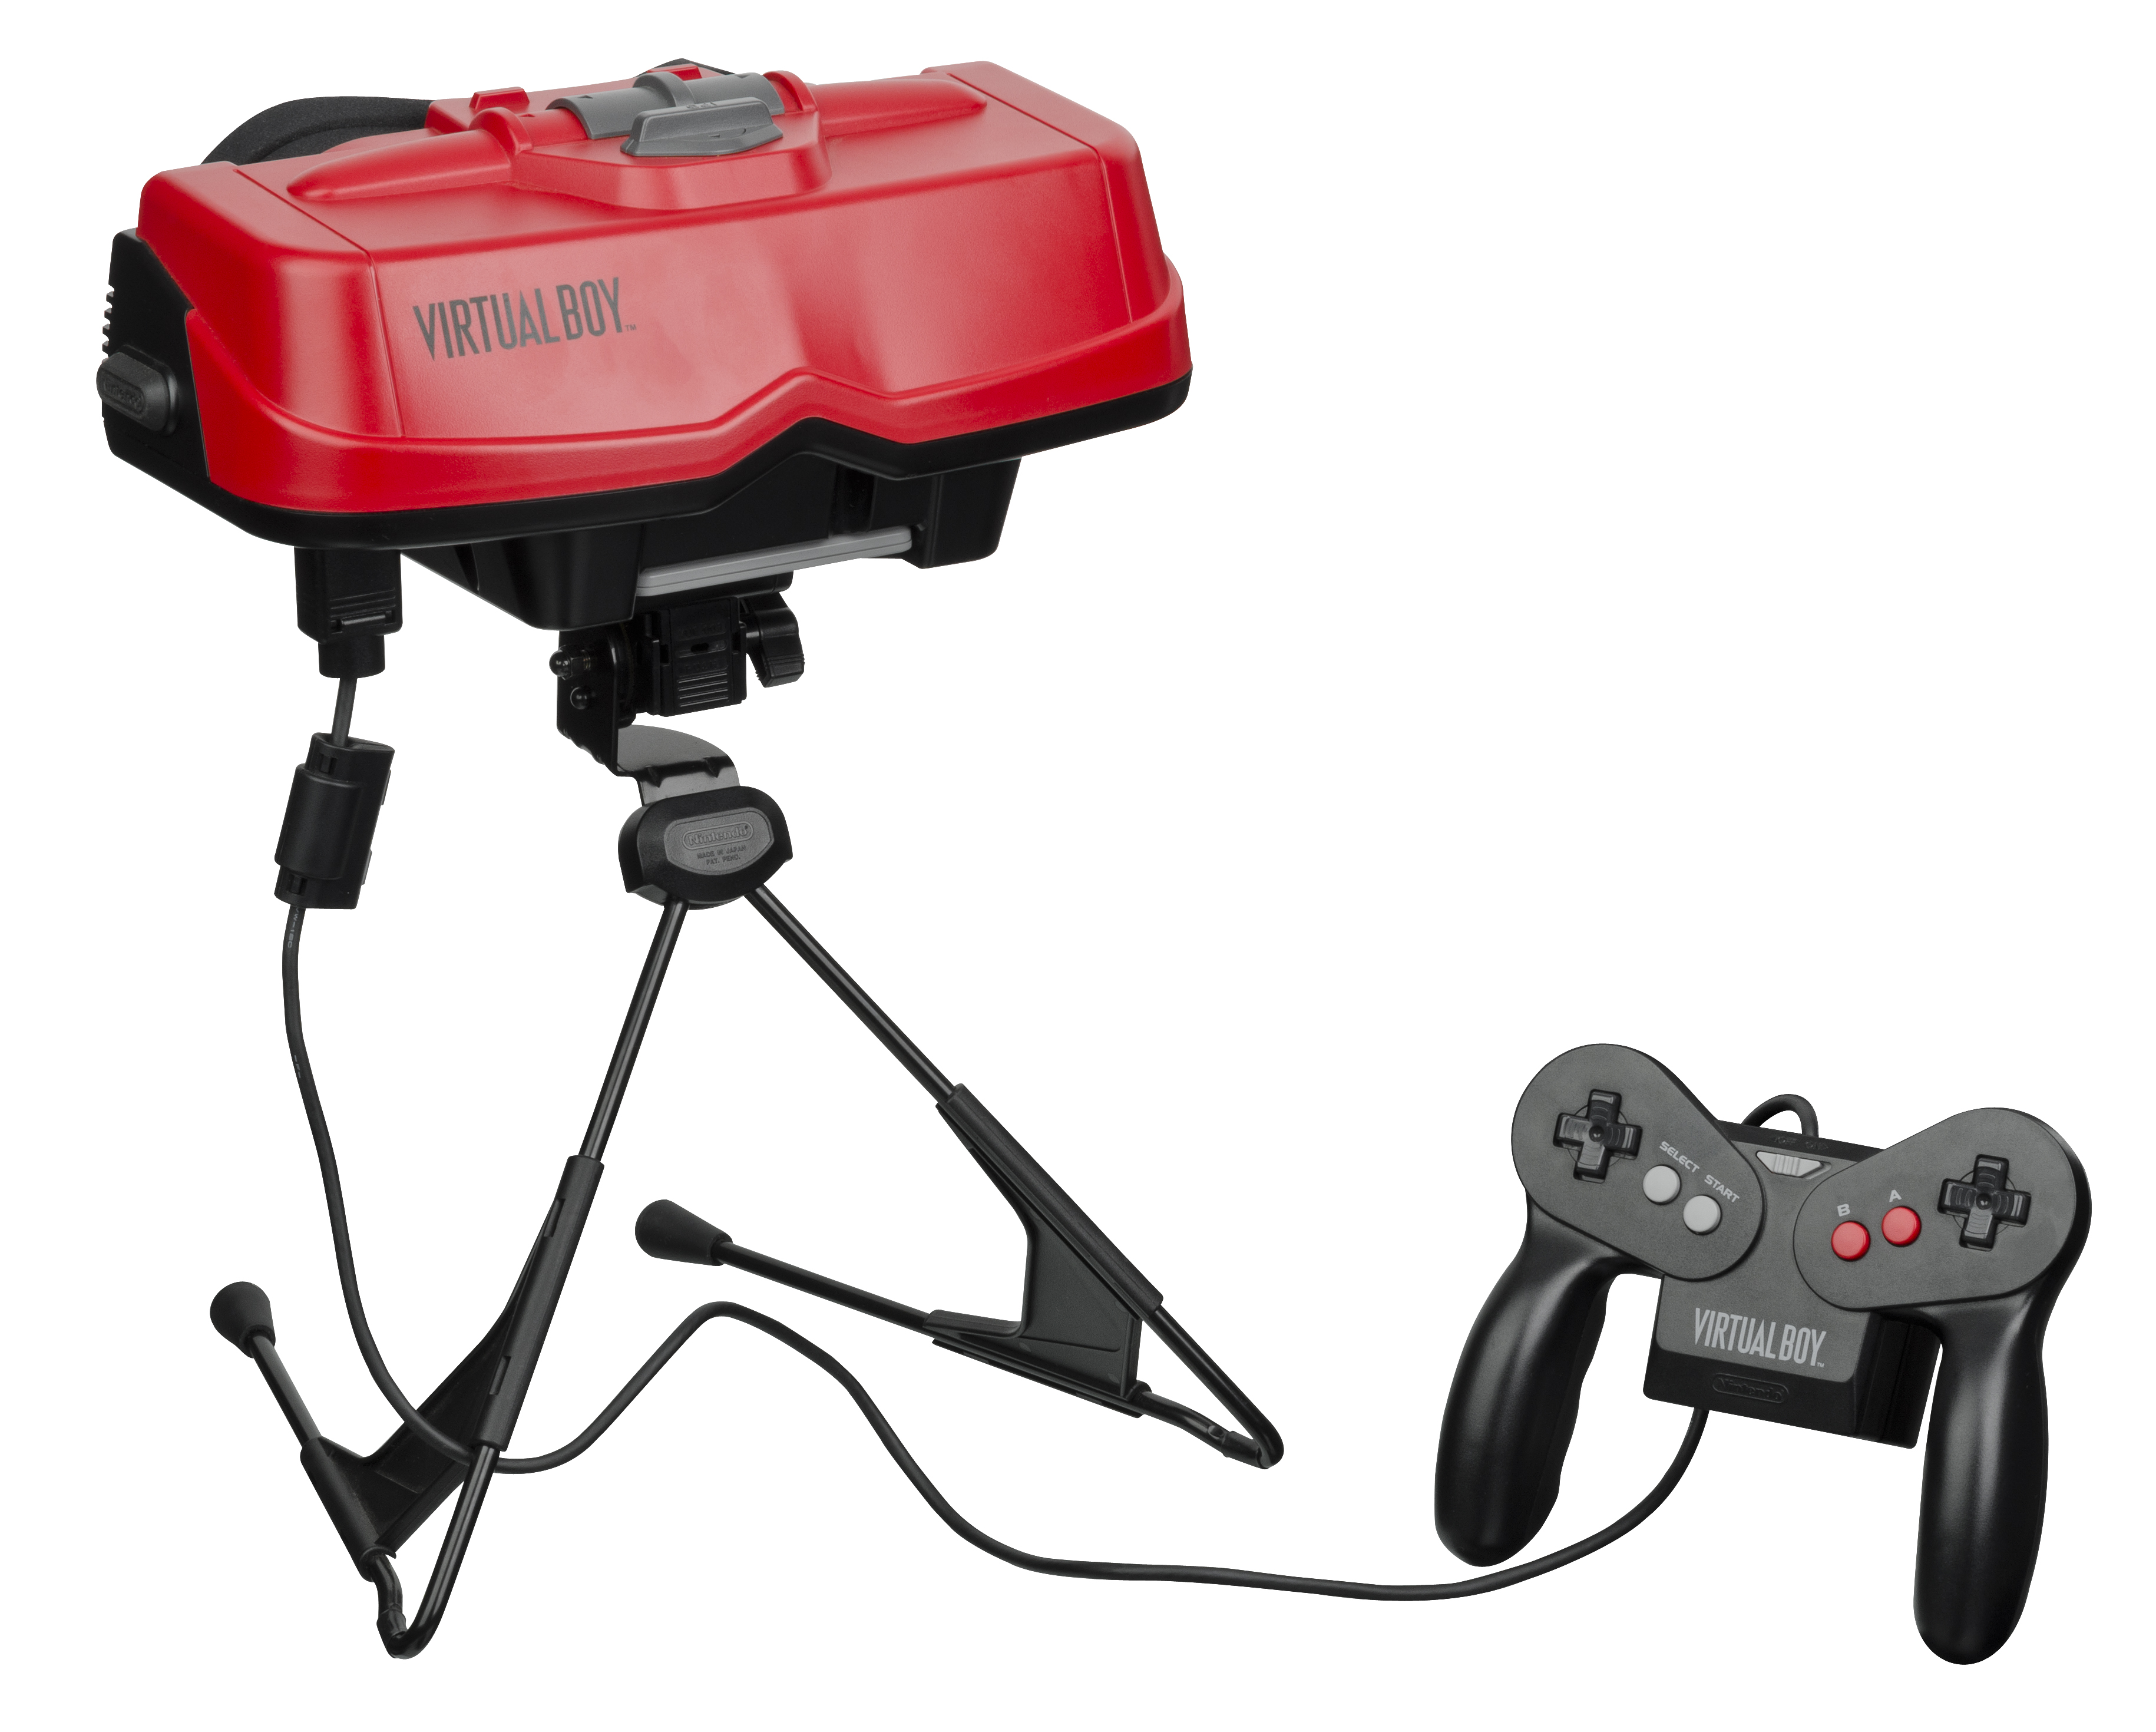
\includegraphics[width=8cm]{src/assets/virtual-boy.jpg}
\caption{Virtuální realita z roku 1995 -- Virtual Boy\autocite{virtualboypic}}
\end{figure}

\section{Virtuální realita v
současnosti}\label{virtuuxe1lnuxed-realita-v-souux10dasnosti}

V současnosti je virtuální realita tvořena typicky pomocí počítačem
generované trojrozměrné grafiky a zvuku, snímání pohybu a snímání polohy
lidského těla. Uživateli je zážitek zprostředkován pomocí náhlavní
soupravy, které vykreslují obraz, přenášejí zvuk a snímají polohu hlavy
uživatele.

V rámci této technologie tak vznikají celé systémy virtuální reality,
které disponují různými vlastnotmi, různými technologiemi simulace a
různou kvalitou simulace. Některé systémy míru a kvalitu simulace
doplňují snímáním celého lidského těla, či částí jejich končetin, např.
ovladačů pro ruce. Snímány mohou být i polohy fyzických předmětů, či
různých jiných ovladačů. 

Systémy se mohou lišit i technologií snímání.
Některé používají infračervené světlo a kamery, jiné zase laserové
snímání. Virtuální realita pro některá mobilní zařízení například
využívá pouze gyroskopických senzorů.

Velkou roli v této technologii hraje, mimo kvalitní a rychlé gyroskopy,
také počítačový výkon. Právě kvůli virtuální realitě začal v poslední
době převažovat trend nových ``VR ready'' počítačových komponent, které jsou
přizpůsobeny k výpočtu obrazu z dvou úhlů pro efekt stereoskopie. \autocite{vrtech}

\section{Systém HTC Vive}\label{systuxe9m-htc-vive}

Systém \emph{Vive} vyvinutý společností \emph{HTC} je jedním z
nejoblíbenějších systémů virtuální reality v současnosti. \autocite{vivepopular} Současně s
\emph{HTC} se na vývoji podílela společnost \emph{Valve}. Tato
společnost stojí za jednou z největších platforem pro digitální
distribuci počítačových her -- \emph{Steam}. S touto službou je úzce
spjatá technologie \emph{SteamVR}. O těchto technologiích více
pojednávají kapitoly níže.

Systém \emph{HTC Vive} se skládá z náhlavní soupravy s OLED displejem o
rozlišení 2160x1200 a dvou ovladačů do ruky s gyroskopickými senzory,
senzory detekce pozice v prostoru, pěti tlačítky, dotykovou plochou a
haptickou odezvou. \autocite{vivespec} Díky laserovému snímání je možné velmi přesně snímat
relativně velký prostor v místnosti, ve které se může uživatel volně
pohybovat. V České republice je k současnému datu systém dostupný za
přibližně 24 tisíc korun. \autocite{viveprice} Koncovým zákazníkům se stal dostupným v dubnu
roku 2016. Pro tento systém bude navržena aplikace této závěrečné práce.

\begin{figure}[h!]
\centering
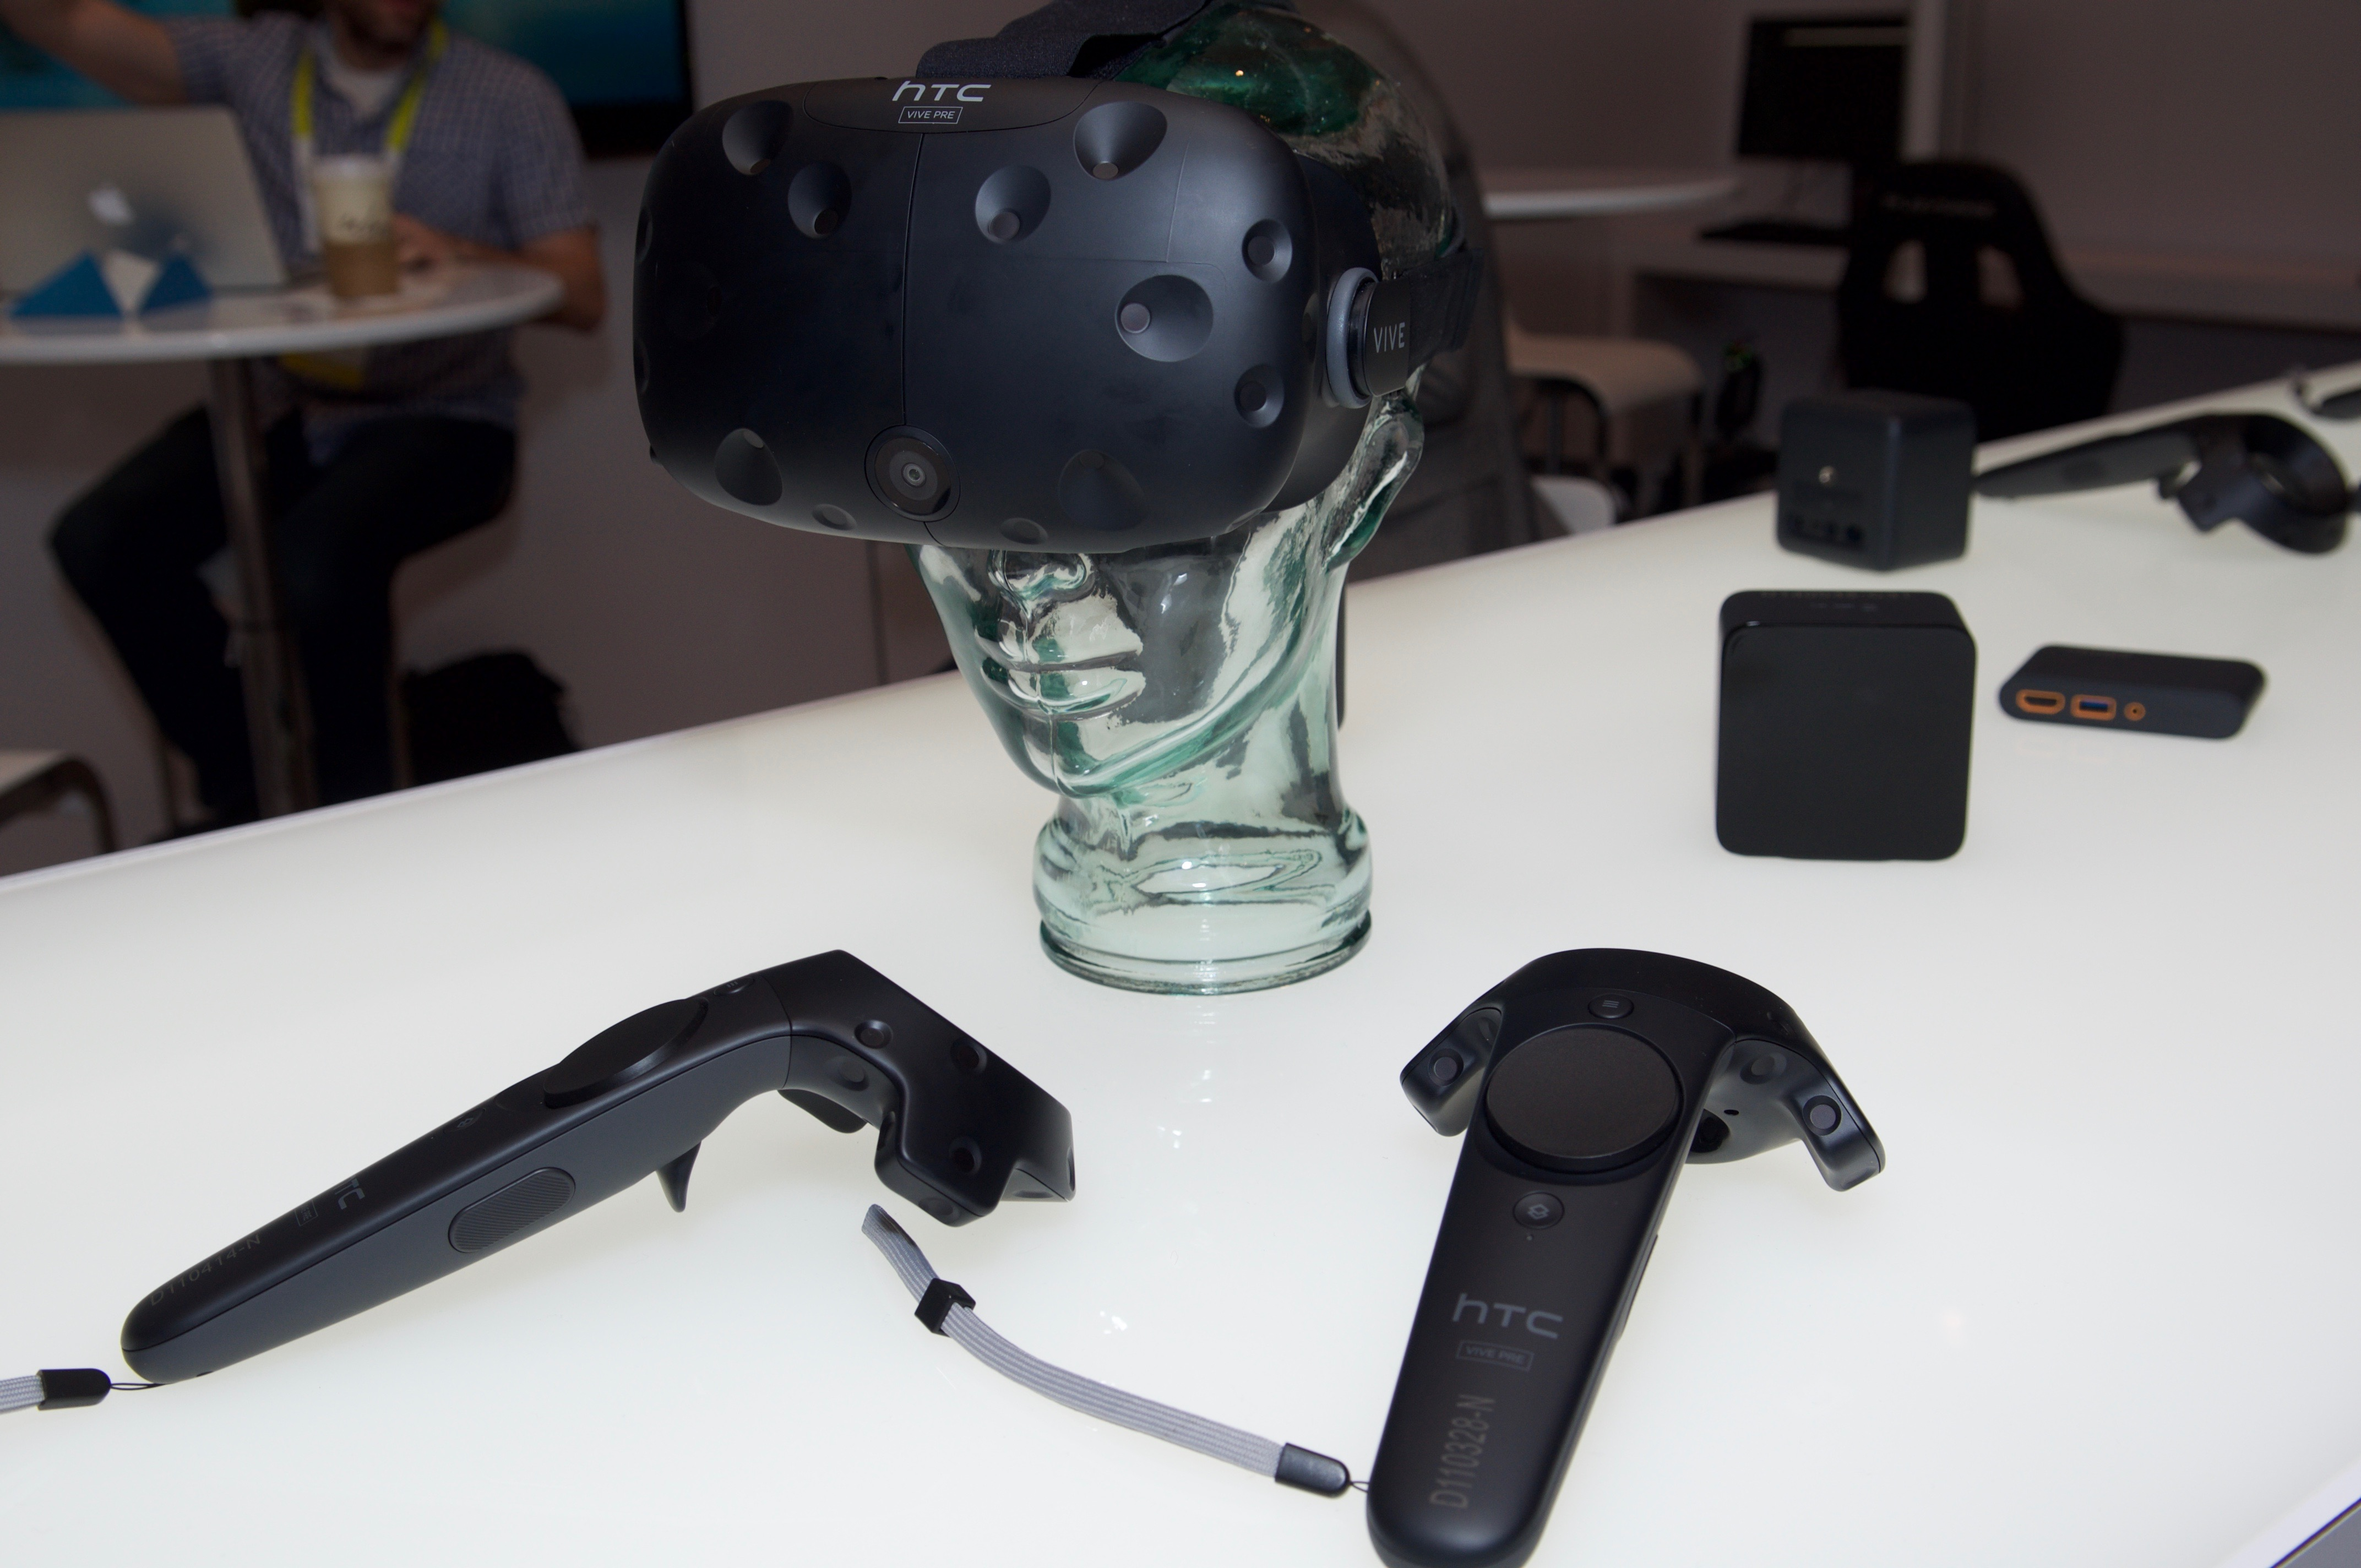
\includegraphics[width=12cm]{src/assets/vive-pre.jpeg}
\caption{Systém virtuální reality HTC Vive a jeho ovladače\autocite{htcvivepre}}
\end{figure}

\newpage

\section{Platforma Steam a SteamVR}\label{platforma-steam-a-steamvr}

Protože se na vývoji systému \emph{HTC Vive} podílela společnost
\emph{Valve}, je více než logické, že \emph{HTC Vive} je úzce spjat s
touto platformou.

Hry a aplikace určené pro tento systém jsou primárně distribuovány skrze
platformu \emph{Steam}. VR aplikace určené pro systém \emph{HTC Vive}
jsou pak podpořeny specializovanou platformou \emph{SteamVR}. Ta je
určena pro práci s hardwarem virtuální reality a jeho komunikaci s
počítačem. Je založena na open-source knihovně \emph{OpenVR}. V současné
době podporuje primárně jen systém \emph{HTC Vive} a v nedávné době byla
přidána experimentální podpora systémů \emph{Oculus Rift} a \emph{OSVR}. \autocite{steamvrsupports}

\emph{SteamVR} má na starosti spojení všech ovladačů a jejich
rozpoznání, a umožňuje systém z počítače ovládat (provést restart či
nastavení). V prostředí virtuální reality pak poskytuje možnost
konfigurace systému, zajišťuje, aby uživatel neopustil vyhrazený prostor
pro pohyb a další podpůrné funkce důležité pro nerušené zážitky ve
virtuální realitě.

\section{OpenVR}\label{openvr}

OpenVR je multi-platformní API rozhraní vyvíjené společností Steam,
které umožňuje snadný a rychlý přístup k hardware virtuální reality
různých výrobců. Poskytuje určitou míru abstrakce k tomu, aby vývojáři
měli přístup k jednotnému rozhraní bez závilosti na tom, jakého výrobce
systém právě používají.

\end{introduction}


\section{Cíl práce}\label{cuxedl-pruxe1ce}

Cílem této závěrečné práce je vytvořit aplikaci usnadňující návštěvníkům
herny seznámení s virtuální realitou a usnadní práci obsluze herny.
Výsledná práce by tak měla nahrazovat klíčové nedostatky systému, na
které lze narazit při použití v prostředí herny.

Aplikace bude rozdělena na dvě části -- výukovou a spouštěč.

Výuková část provede uživatele vstupem do virtuální reality. Bude mu
představeno prostředí, ve kterém se bude pohybovat a budou mu
představeny ovladače systému \emph{HTC Vive}, pro který je tato aplikace
primárně určena. Návštěvník herny tak bude v co nejkratším čase zaučen a
zefektivní se i práce obsluhy herny. Zatímco návštěvník prochází výukou,
obsluha se může začít věnovat dalším zákazníkům herny.

Po ukončení výuky bude pomocí vlastního spouštěče představena nabídka
titulů, které si může uživatel v herně vyzkoušet. Knihovna her a
aplikací bude taktéž kategorizována a bude zobrazovat oblíbené tituly,
které herna dopouručuje, či ty tituly, které jsou v herně oblíbené.
Funkce tak nahrazuje dotazovat se návštěvníků, co mají rádi a odhadovat
tak o jaký typ zážitku by mohli mít zájem.

Výstupem bude analýza současného stavu, návrh aplikace pro výuku a
doplňkové aplikace spouštěče a následně samotná realizace takové
aplikace.

Mezi plánované klíčové vlastnosti aplikace je zařazena efektivita výuky,
kvalitní vizuální zpracování a nízká obtruzivnost aplikace. Je nutné
myslet na to, že aplikace bude nasazena v prostředí, kde uživatelé
disponují limitovaným časem. Zakoupili si omezený čas zápůjčky systému a
aplikace by je neměla o jejich zakoupený čas připravit.

\chapter{Analýza}\label{analuxfdza}

Jak je zvykem u organizovaného vývoje softwaru -- implementaci a návrhu
aplikace předchází analýza, pro stanovení požadavků uživatelů softwaru a
upřesnění funkcionalit aplikace.

Následující kapitola se takovou analýzou bude zabývat. Budou analyzována
existující řešení, zjištěno, co požadují návštěvníci herny a
zaměstnanci pracující v herně, a jaké požadavky jsou realizovatelné.

\section{Analýza a porovnání existujících řešení
výuky}\label{analuxfdza-a-porovnuxe1nuxed-existujuxedcuxedch-ux159eux161enuxed-vuxfduky}

Výukové aplikace pro seznámení s virtuální realitou již existují.
Nicméně většina z nich trpí špatnou přístupností. Jsou navrhovány tak,
že po absolvování takové výuky již nejsou jednoduše dostupné. Jsou tak
obtížně spustitelné pro návštěvníky herny.

Takové aplikace jsou spíše určené pro toho, kdo jako první systém
konfiguruje a je jeho prvním uživatelem. Nově příchozímu k
nakonfigurovanému systému není tutoriál nabídnut a je přímo uveden do
prostředí, ve kterém se již očekává, že uživatel systém důvěrně zná.

Součásti analýzy je i porovnání jednotlivých existujících řešení, pro
které jsou stanoveny následující metriky k porovnání:

\begin{itemize}
\tightlist
\item
  jednoduchost přístupu k výukové aplikaci
\item
  rychlost a svižnost výuky
\item
  zábavnost
\item
  výstižnost
\item
  srozumitelnost
\end{itemize}

\subsection{SteamVR Tutorial}\label{steamvr-tutorial}

Pro totožnou platformu, pro kterou je aplikace této závěrečné práce
určena existuje oficiální výuková aplikace vytvořená přímo společností
\emph{Valve}.

\subsubsection{Průběh výuky}\label{prux16fbux11bh-vuxfduky}

Aplikace se nejprve uvede vizuálně poutavým úvodem, který spočívá v
sestavení výukové scény animací obklopující uživatele. Uživateli je tak nenuceně
ukázána možnost rozhlížet se kolem sebe a prozkoumávat prostředí, což
většina uživatelů intuitivně udělá.

Následně je uživateli představena postava \emph{Virtual Reality
Assistance and Education Core} z prostředí hry Portal 2, která s uživatelem
komunikuje a provádí ho výukou -- stává se tak \emph{průvodcem}. Monolog
je dabovaný a v místech, kde se nachází průvodce se zobrazují titulky,
které jsou lokalizovány do nepřeberného množství jazyků (i češtiny).

Příjemným bonusem je pro hráče hry Portal 2 familiarita postavy, která
může zvýšit pozornost, a pro hráče, kteří si hru Portal 2 v
minulosti oblíbili, tak tutoriál navozuje na obličejích úsměv.

\begin{figure}[h!]
\centering
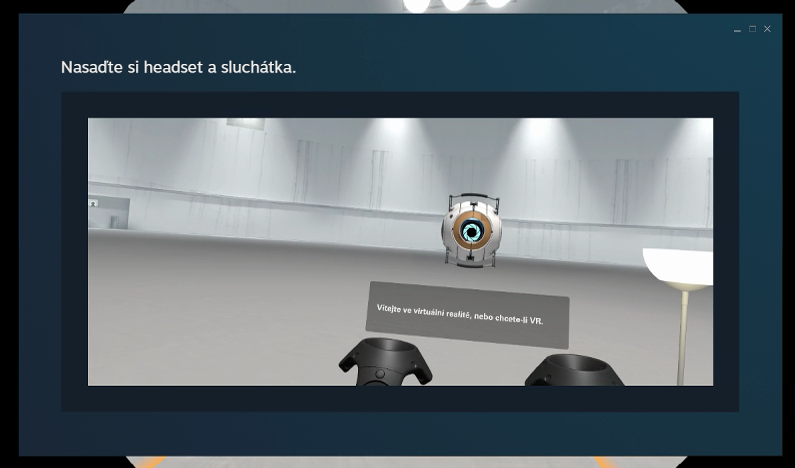
\includegraphics[width=12cm]{src/assets/steamvr-tutorial.png}
\caption{Výuková aplikace SteamVR Tutorial}
\end{figure}

Jako první je uživateli představena plocha, tzv. \emph{play area}, ve
které se VR zážitky budou odehrávat. Neprodleně jsou pak představeny
tzv. \emph{chaperone bounds}, které upozorňují na skutečnost opouštění 
hranice \emph{play area}. Protože je tato funkcionalita
důležitá pro jeho bezpečnost, je na ni ve výuce kladen důraz a je proto
požádán, aby se ke kraji místnosti pomalu přiblížil a následně to stejné
zopakoval na druhé straně místnosti.

Dále je uživatel požádán, aby se podíval na ovladače, které drží v ruce
a provedl s nimi libovolné pohyby pro vyzkoušení manipulace.
Poté, co se seznámí s pohyby s ovladačem jsou mu postupně představena
všechna tlačítka, která se na něm nacházejí a je požádán, aby každé
stiskl a vyzkoušel si, kde se nacházejí a jakou mají zpětnou odezvu.

Výuková aplikace je pojatá spíše komicky a každé tlačítko velmi chytře
vyvolává různé destrukční, hlasité a nečekané události, které se
průvodci příliš nelíbí. Průvodce uživatele po chvíli žádá, aby s opakovaným
mačkáním přestal. Uživatel však může mít zlé úmysly a nutkání tyto tlačítka
stisknout opakovaně, aby průvodce rozčílil a dělal nepořádek. Tím se
však s tlačítky seznámí o to více.

Uživatel není informován o tom, která tlačítka mají jakou funkci, logicky z
důvodu, že každá VR aplikace má své vlastní pojetí smyslu těchto
tlačítek. Ovšem k tlačítkům \emph{Menu} a \emph{System} je uživateli
řečeno, k čemu se nejčastěji používají.

Uživatel je požádán o stisk tlačítka \emph{System}, což vede k otevření
\emph{SteamVR Dashboard}. Lze si povšimnout, že se výuka při oteření
nepozastaví, a probíhá tak stále instruktáž, jak se lze ve \emph{SteamVR
Dashboard} pohybovat a k čemu je určena.

Tím je výuka u konce. Uživatel je instruován k otevření
\emph{Dashboardu} (pokud jej opustil) a výběrem VR aplikace. Může však v
aplikaci zůstat a dále zkoušet práci s ovladači, nebo zhlédnout
závěrečnou animaci, kdy průvodce komicky odvezou jiné postavy pryč ze
scény. \autocite{steamvrshuts}

\subsubsection{Zhodnocení}\label{zhodnocenuxed}

SteamVR Tutorial je dobrým příkladem výukové aplikace. Je kvalitně
navržena, spíše se strohým, ale kvalitním vizuálním a zvukovým
zpracováním.

Pro účely herny je však shledána za nevhodnou, jelikož je návštěvníkům herny
taková aplikace prakticky nepřístupná. Obsluha je nucena ji spustit
manuálně a také se návštěvníka herny zeptat, jestli už výuku absolvoval
a zda ji chce skutečně absolvovat. Návštěvník nemá možnost si takovou
výuku spustit sám, zopakovat ji, nebo alespoň po absolvování získat
nějaký závěrečný přehled, pro zopakování toho, co se naučil.

\begin{figure}[h!]
\centering
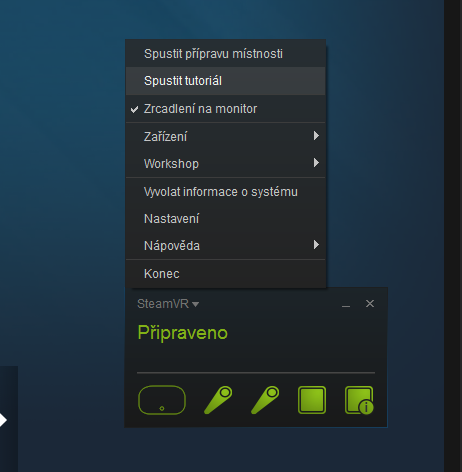
\includegraphics[height=8cm]{src/assets/hidden-menu.png}
\caption{Přístup k aplikaci je skryt ve SteamVR nabídce, která je
přístupna jen z monitoru počítače}
\end{figure}

Další nevýhodou je délka tutoriálu, která se běžně pohybuje kolem 6-11
minut. To představuje v prostředí, kde se běžně systém zapůjčuje na
jednu hodinu, velkou část herního času.

\subsection{Oculus Touch Tutorial \& Oculus First
Contact}\label{oculus-touch-tutorial-oculus-first-contact}

Pro konkurenční systém \emph{Oculus Rift} a jeho platformu je určena
aplikace \emph{Oculus First Contact}, která je spojena s předcházející
krátkou výukou k ovladačům \emph{Oculus Touch}, které jsou k systému
\emph{Oculus Rift} prodávány odděleně. Bez těchto ovladačů tuto výuku
nelze absolvovat.

\subsubsection{Průběh výuky}\label{prux16fbux11bh-vuxfduky-1}

Uživatel je zasazen do čistého prostředí, bez předmětů, zobrazující
pouze ovladače v ruce. Před ním se pak zobrazuje přepis (titulky) hlasu
průvodkyně, která není vizuálně zpracována, lze slyšet pouze hlas.

Jako první je požádán, aby se podíval na podlahu a zpozoroval obrys
prostoru, ve kterém se může uživatel pohybovat (\emph{play area}).
Následně je požádán, aby se podíval na své ruce a ovladače, které drží,
a osahal si všechna tlačítka, která se mu podaří nalézt. Následně jsou
mu všechna tlačítka jedno po druhém představeny. Jsou postupně
zvýrazněny a je požádán, aby tato tlačítka stiskl.

\begin{figure}[h!]
\centering
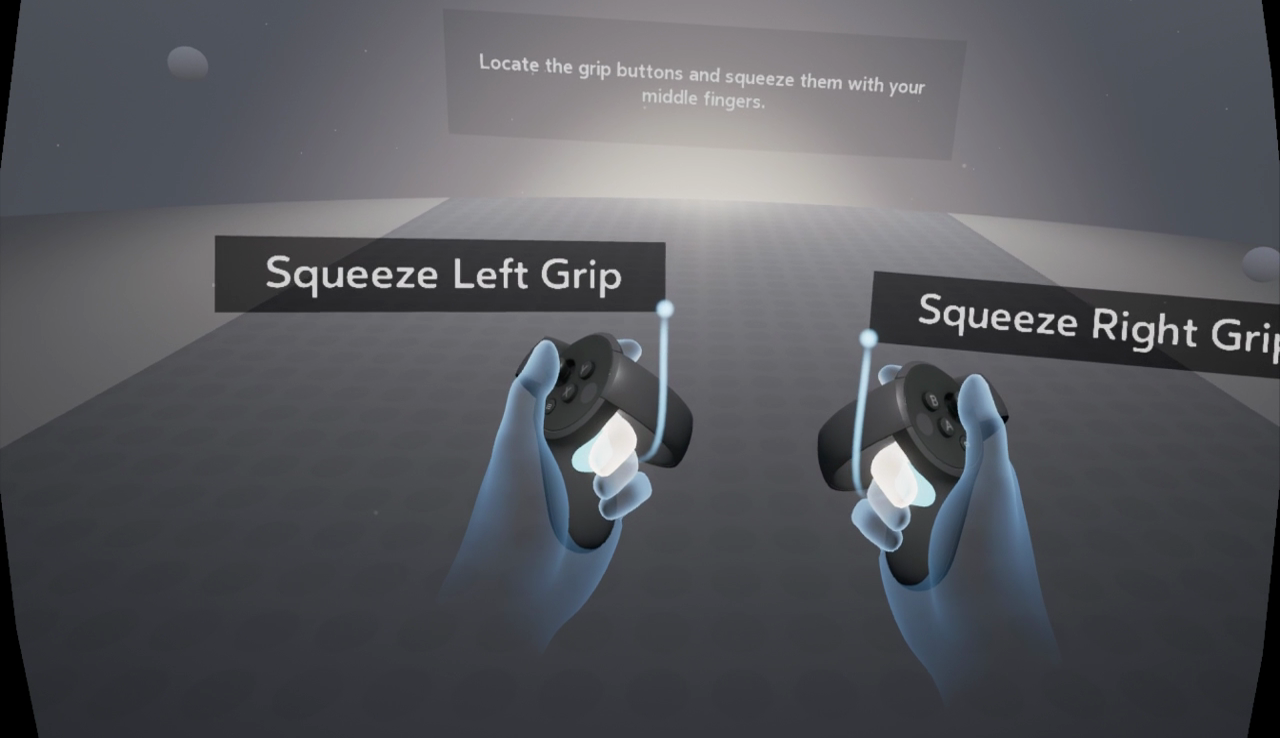
\includegraphics[width=12cm]{src/assets/oculus-tutorial.png}
\caption{Výuková aplikace Oculus Touch Tutorial}
\end{figure}

Pokud uživatel provádí stisky tlačítek svižně, lze tuto část projít
rychleji. Výuka nezdržuje dlouhým monologem nebo pauzami. Jde o krátké
věty a díky tomu působí velmi svižně.

Vzápětí jsou uživateli ovladače vizuálně z rukou odstraněny a je
požádán, aby znovu vyzkoušel stisknout tlačítka a zvedat z nich prsty
tak, aby pochopil reprezentaci přirozeného pohybu rukou a prstů, kterou
se ovladače \emph{Oculus Touch} od konkurence liší. 

Je požádán, aby
stiskl specifické kombinace tlačítek takovým způsobem, aby vytvářel
gesta rukou, jako je například gesto uzavření v pěst nebo míření na
objekty ukazováčkem.

Uživateli není vysvětlen účel tlačítek, z dříve zmíněných důvodů. Pokud
však předpokládáme, že všechny VR aplikace a hry budou implementovat
systém gest ruky, které byly vysvětleny v třetí části výuky, uživatel je
schopen odvodit účel tlačítek sám, což lze považovat za nespornou
výhodu.

Překvapující je absence objasnění smyslu tlačítek \emph{Oculus} a
\emph{Menu}, které většinou ve všech VR aplikacích mají totožný účel.

Tím výuka končí a je spuštěna aplikace \emph{Oculus First Contact},
která je určena k prohloubení právě nabytých znalostí, a slouží jako
úvodní zábavný zážitek, který je srovnatelně kvalitní a zábavný jako
jiné herní tituly pro virtuální realitu. Tím tak lze považovat výuku
za dokončenou a aplikací \emph{Oculus First Contact} začíná
``zábava''.

\begin{figure}[h!]
\centering
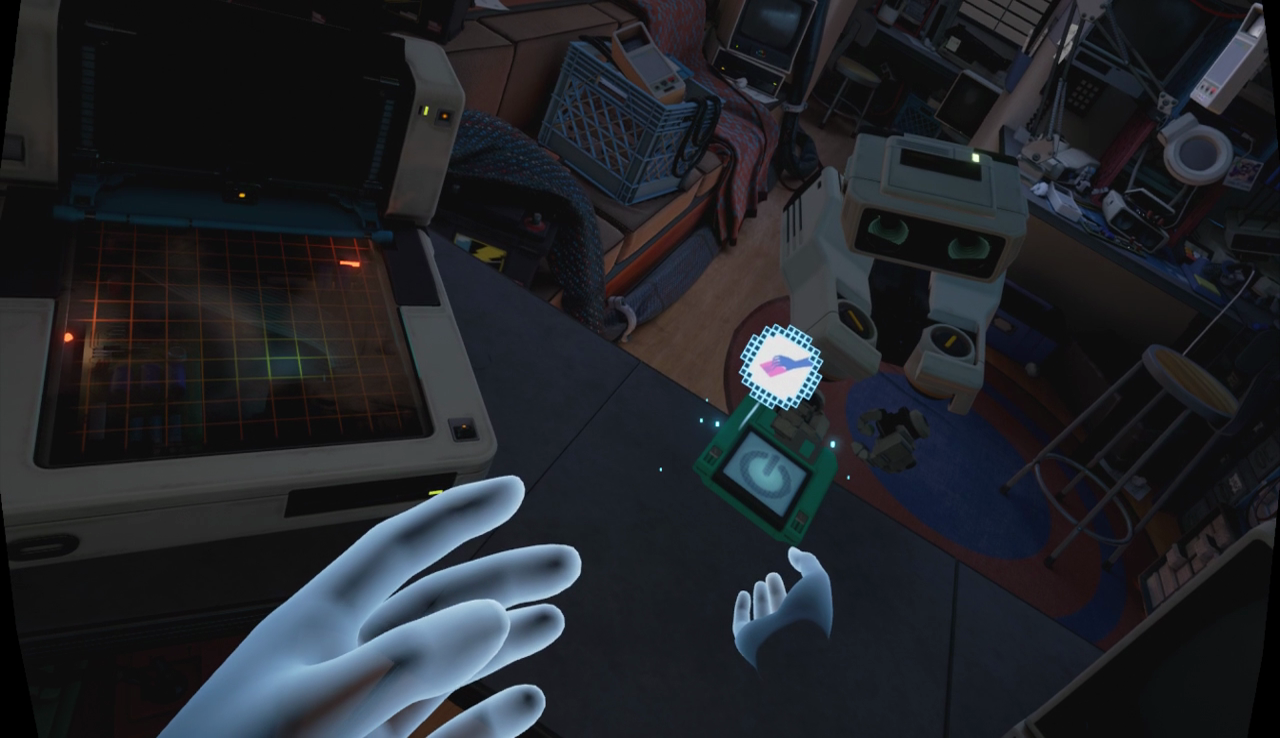
\includegraphics[width=12cm]{src/assets/oculus-first-contact.png}
\caption{Aplikace Oculus First Contact}
\end{figure}

\subsubsection{Zhodnocení}\label{zhodnocenuxed-1}

\emph{Oculus} má výukovou aplikaci zpracovanou do podstatně rychlejšího
tempa, než \emph{SteamVR}. Přispívá tomu i jednoznačné rozdělení výuky
od zábavy. Nejprve přichází rychlý a strohý úvod ovládání, který trvá
přibližně 4-5 minut. Až následně po tomto úvodu následuje zábavný prvek
ve formě plnohodnotného VR zážitku. Vidíme tak zásadní rozdíl oproti
SteamVR, který tyto dva prvky míchá do jednoho spojeného průběhu.

\section{Analýza existujících řešení
spouštěčů}\label{analuxfdza-existujuxedcuxedch-ux159eux161enuxed-spouux161tux11bux10dux16f}

Po skončení výuky můžeme předpokládat, že návštěvník herny je se
systémem do určité míry seznámen a dále je nutné mu nějakým způsobem
nabídnout výběr VR zážitků. O VR aplikacích může mít předchozí znalost a
jít do herny za účelem konkrétní aplikaci vyzkoušet, nebo může hernu
navštívit, protože chce zkrátka vyzkoušet virtuální realitu. Druhý
zmíněný důvod je v hernách vídán mnohem častěji.

Dvě v předchozí kapitole zmíněné platformy (SteamVR a Oculus) mají
vlastní software pro spouštění VR aplikací. Ty jsou v této kapitole
analyzovány.

\subsection{SteamVR Dashboard}\label{steamvr-dashboard}

\emph{SteamVR Dashboard} je pouze malou modifikací již existujícího
\emph{Steam Big Picture} -- rozhraní pro práci s platformou
\emph{Steam}, které je přizpůsobeno pro ovládání herním ovladačem.

U hráčů počítačových her je velká pravděpodobnost, že se s platformou
\emph{Steam} již v minulosti setkali. Mnozí z nich se také setkali i s
rozhraním \emph{Big Picture}, které někteří dokonce používají jako
primární rozhraní pro práci s platformou \emph{Steam}. Tento fakt
představuje nespornou výhodu, protože takoví hráči se budou pohybovat ve
známém prostředí.

Na druhou stranu lze však považovat jako nevýhodu fakt, že \emph{Steam
Big Picture} nebyl původně navržen pro použití s VR. Uživatel tak pracuje s
malým oknem na virtualizovaném monitoru. Vidí před sebou plochu, na
kterou je rozhraní plošně promítáno. Není tak plně využito potenciálu VR
prostoru.

\begin{figure}[h!]
\centering
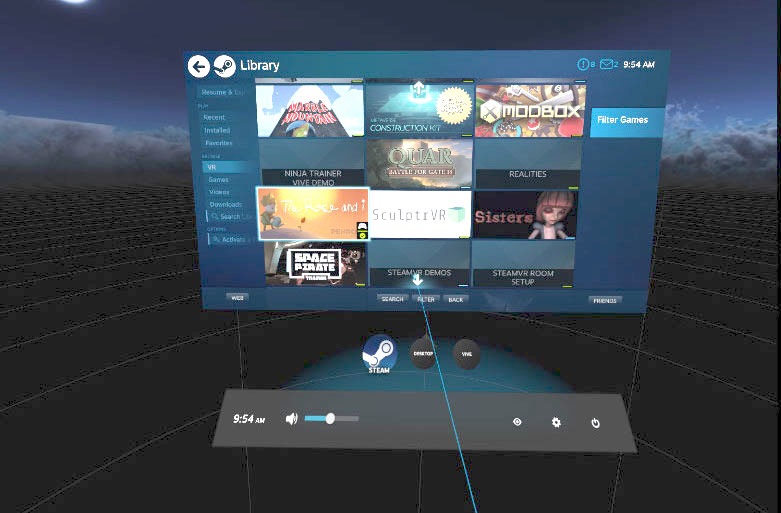
\includegraphics[width=12cm]{src/assets/steamvr-library.jpg}
\caption{SteamVR Dashboard \autocite{tomshardw}}
\end{figure}

Z tohoto rozhraní lze procházet knihovnu her, prohlížet elektronický
obchod s hrami, nakupovat v něm, prohlížet komunitní profily, stránky
her, sledovat průběh aktuálního stahování, používat webový prohlížeč,
zobrazit monitor počítače, ovládat počítač a přistupovat k nastavení.

Pokud budeme hodnotit \emph{SteamVR Dashboard} z pohledu návštěvníka
herny, je takové rozhraní nevyhovující. Pro návštěvníka, který nemá s
platformou \emph{Steam} zkušenosti je rozhraní spíše matoucí a může
vyžadovat určitou dobu, než se s ním seznámí. 

V rozhraní se nacházejí
sociální a komunitní funkce, které pro použití v herně nemají žádný
význam a jsou dalším matoucím prvkem pro návštěvníka. Dále je poskytnut
plný přístup k obchodu a kdokoliv by mohl na účet herny libovolně
nakupovat hry. Není mu v tom nikterak zabráněno.

Seznam a výběr VR aplikací je pro použití v herně taktéž spíše nevhodný.
Seznam se skládá z mřížky 3x4 grafických bannerů, které o dané hře, či aplikaci 
vypovídají jen málo. Je totiž na vývojářích, či v takovém banneru
zobrazí pouze logo, obrázek z aplikace, či obojí. Lze tak velmi obtížně
odhadnout o jaký žánr hry či typ aplikace jde, zda je zábavná, vizuálně přitažlivá, jaké
ovládání podporuje či zda způsobuje závratě a kinetózu.

\subsection{Oculus Home}\label{oculus-home}

\emph{Oculus Home} je plnohodnotným rozhraním pro virtuální realitu od
společnosti Oculus pro svou stejnojmennou platformu. Narozdíl od
\emph{SteamVR Dashboard} je navržen přímo pro VR.

Skrze toto rozhraní lze procházet knihovnu her a aplikací, či nakupovat hry v
obchodě. Uživatel může vidět i minimální komunitní funkce, jakými jsou
seznam hráčů a notifikace (a to i systémové).

Rozhraní je vizuálně velmi přitažlivé. Zobrazuje se jako výchozí prostor
při nasazení headsetu na hlavu bez spuštěné aplikace, což oproti platformě
SteamVR, kde se zobrazuje prázdná šedá místnost s mřížkou, působí lepším
dojmem.

\begin{figure}[h!]
\centering

\includegraphics[width=12cm]{src/assets/oculus-home.png}
\caption{Oculus Home}
\end{figure}

Jelikož je rozhraní navržené specificky pro použití s aplikacemi pro
virtuální realitu, k hrám lze nalézt informace o tom, jaké ovladače
podporuje a lze je řadit podle míry ``komfortu''. Nekomfortní hry a aplikace jsou
pak označeny jako takové, které mohou způsobovat kinetózu. Díky tomu se
lidé, kterým se z intenzivnějších zážitků dělá nevolno, mohou snadno takovým
hrám či aplikacím vyhnout.

V prostředí herny je však \emph{Oculus Home} také mírně nevyhovující.
Přístup k obchodu a komunitní funkce jsou irelevantní účelu herny a
zbytečně odvádějí pozornost.

\section{Pozorování v herně}\label{pozorovuxe1nuxed-v-hernux11b}

Ke konci března roku 2017 se naskytla příležitost stát se na jeden den
obsluhou v herně \emph{Virtualnirealita.cz} v pražských Dejvicích. Tato
příležitost byla využita v prospěch analýzy, jako předmět pozorování a
bližšího pochopení požadavků zákazníků a obsluhy herny.

Jako obsluha vznikala povinnost seznámit zákazníky s pronajatým
systémem. Pokud s virtuální realitou neměli dosud zkušenost, nebo se
nedoslechli o žádné konkrétní VR aplikaci, kterou by si přišli
vyzkoušet, bylo nutné doporučit nějakou VR aplikaci na základě jejich
preferencí.

Aby bylo možné se zákazníky lépe pracovat a doporučit jim správnou
aplikaci, byli dotazováni na přirozené otázky. Z odpovědí na ně vznikla
miniaturní analýza z malého vzorku lidí, kteří ten den hernu navštívili.

Dotazování zákazníků se tak běžně skládalo z otázek: 

\begin{itemize}
\tightlist
\item
``Už jste u nás
někdy byli?''
\item
  ``Máte zkušenosti s VR?''
\item
  ``Hrajete počítačové hry?''
\item
  ``Jaký žánr her rádi hrajete?''
\end{itemize}

Za daný den navštívilo hernu \textbf{15 zákazníků}, z toho \textbf{10
mužů}. Většina -- \textbf{12 zákazníků} hraje počítačové hry, ale pouze
\textbf{2 z nich} v minulosti hernu navštívili, nebo měli s VR
zkušenost. Většina z nich byla mládež (v rozmezí 15-30 let), výjimku
tvořili \textbf{2 děti} (\textless{} 15) a \textbf{2 dospělí}
(\textgreater{} 30). U jednoho ze zákazníků se projevila
\emph{kinetóza}.

Pouze \textbf{4 z nich} odpověděli, že jim nepřišly ovladače systému HTC
Vive obtížné na seznámení, stejně tak tito lidé odpověděli, že by se
obešli bez pomoci obsluhy. Dva z těchto čtyř byli ti, kteří již s VR
měli zkušenost.

Občasným jevem bylo několikanásobné vystřídání zákazníků na jednom
systému za dobu zapůjčení. To je důležitá informace, protože výuková
aplikace musí s takovým jevem počítat. Rychlost seznámení se systémem
byla převážně ovlivněna zákazníkovou zkušenosti s počítačovými hrami.

\section{Funkční požadavky zákazníků
herny}\label{funkux10dnuxed-poux17eadavky-zakazniku-herny}

Z pozorování v herně a analýzy existujících řešení plynou následující
požadavky vztahující se k zákazníkům herny.

\subsubsection*{F-A01 Uživatel se chce seznámit se základními pravidly systému
virtuální reality}
Uživatel chce vědět, jak se používá headset systému virtuální reality,
jak se může v \emph{play area} pohybovat, kam se nesmí vydat a jak je na
to upozorněn. Funkční požadavek je klíčový z hlediska bezpečí
návštěvníka herny a ochrany majetku herny.

\subsubsection*{F-A02 Uživatel se chce seznámit s ovladači a jejich tlačítky}
Uživatel chce vědět, jak vypadají ovladače, jakými tlačítky disponují a
k čemu slouží. V závislosti na této znalosti je pak uživateli usnadněno
pochopení ovládání v konkrétních VR aplikacích.

\subsubsection*{F-A03 Uživatel se chce seznámit s funkcemi na tlačítkách pro
konkrétní hru}
Uživatel chce vědět, jak se ovládá konkrétní VR aplikace.

\subsubsection*{F-A04 Uživatel si chce vybrat VR aplikaci podle žánru}
Uživatel si chce zvolit VR zážitek takového žánru, který mu vyhovuje. Do
herny docházejí různé věkové a zájmové skupiny. Často záleží i na
pohlaví. Ženy většinou rády hrají méně intenzivnější zážitky, vyhýbají
se hororovým hrám a ``střílečkám'' a více ocení vizuálně atraktivní
aplikace. \autocite{ladiespreferences}

\subsubsection*{F-A05 Uživatel si chce vybrat VR aplikaci podle intenzity}
Uživatel, u kterého se projevuje kinetóza, si chce vybrat takovou
aplikaci, aby nebyla příliš intenzivní a jeho zážitek z VR byl
pozitivní. Ač může být toto kritérium velmi subjektivní, lze aplikace
rozdělit alespoň do dvou kategorií, jako intenzivní a klidné, kde pod
klidné aplikace spadají všechny aplikace, které mají implementovány
mechanismy zabraňující kinetóze, nebo nezahrnují pohyb kamery kinetózu
způsobující.

\subsubsection*{F-A06 Uživatel si chce vybrat VR aplikaci podle vizuálního
zpracování}
Uživatel si chce vybrat takovou aplikaci, která bude pro něj vizuálně
atraktivní. Spousta uživatelů upřednostňuje určité aplikace z
jednoduchého důvodu -- líbí se jim.

\subsubsection*{F-A07 Uživatel chce výuku kdykoliv přeskočit, nebo informace
zopakovat znova} 
Pokud uživatel shledá výuku subjektivně příliš
jednoduchou, či zdlouhavou, měl by mít možnost její průběh minimálně
urychlit. Naopak, pokud je pro něj výuka příliš rychlá, měl by mít na
konci výuky možnost si informace zopakovat, či zopakovat celou výuku
znova.

\subsubsection*{F-A08 Uživatel chce, aby byla výuka časově efektivní}
Protože má zákazník herny omezený čas, po který je mu zapůjčen systém
virtuální reality, je pro něj důležité, aby ho výuka o tento čas
připravila v co nejmenší míře.

\section{Funkční požadavky obsluhy
herny}\label{funkux10dnuxed-poux17eadavky-obsluhy-herny}

Požadavky obsluhy se velkou částí kryje s požadavky zákazníka, jen z
jiného úhlu pohledu.

\subsubsection*{F-B01 Obsluha chce zákazníka seznámit s pravidly používání
systému virtuální reality}
Aby uživatel používal systém správně, obsluha se potřebuje ujistit, že
zákazník ví, jak se systém používá, aby nedošlo k jeho poškození
nesprávným použitím a zákazník nebyl vystaven nebezpečí.

\subsubsection*{F-B02 Obsluha chce zákazníka seznámit s ovladači systému}
Aby uživatel byl se zážitkem spokojený, obsluha potřebuje, aby zákazník
byl schopen používat ovladače systému. Taková znalost pak zákazníkovi
usnadní pochopení ovládání konkrétních aplikací a je tak logicky více
spokojený.

\subsubsection*{F-B03 Obsluha chce, aby si zákazník vybral VR aplikaci pro něj
vhodnou}
Zákazníci velmi často přicházejí do herny pouze za účelem vyzkoušení
virtuální reality. Zřídkakdy se stává, že by zákazník věděl o jakou
konkrétní VR aplikaci má zájem a chce si ji vyzkoušet. Obsluha je tak
povinna zjistit, co bude zákazníkovi vyhovovat a vybrat mu tak nějakou
aplikaci či herní titul pro něj vhodný.

\subsubsection*{F-B04 Obsluha chce zákazníka upozornit na blížící se konec
vypůjčení systému}
Přibližně pět minut před koncem doby zápůjčky obsluha žádá zákazníka,
aby si na moment sundal sluchátka, aby jej mohla upozornit na blížící se
konec.

\section{Funkční požadavky
obecné}\label{funkux10dnuxed-poux17eadavky-obecnuxe9}

Požadavky nekategorizovatelné jako požadavek zákazníka či obsluhy
herny. Většina z nich se týká fukncionality spouštěče.

\subsubsection*{F-C01 Uživateli je zobrazen seznam VR aplikací a je mu umožněn
výběr}
Základní funkce spouštěče je zobrazení seznamu VR aplikací, ze kterých
může uživatel provést výběr. Takový seznam by měl poskytovat možnost
vyhledávat přímo podle názvu, dále podle žánru, intenzity i podle
vizuálu.

\subsubsection*{F-C02 Uživateli jsou zobrazená podrobnější data k VR aplikaci}
Aby mohla aplikace splnit požadavek \emph{F-C01}, je nutné taková data o
hrách získat. Většina požadavkem zmíněných dat je dostupná přes veřejná
API. Více se získáním dat bude zabývat \ref{nuxe1vrh}.

\subsubsection*{F-C03 Spustí se uživatelem vybraná VR aplikace}
Poté, co uživatel provede výběr aplikace, je tato aplikace spuštěna a
funkce spouštěče jsou pozastaveny či ukončeny.

\subsubsection*{F-C04 Po ukončení VR aplikace je uživateli znovu nabídnut
přehled her a aplikací}
Po ukončení práce s VR aplikací, kterou uživatel spustil, je mu opět
nabídnut výběr spouštěče (pokračováním v činnosti či opětovým
spuštěním).

\section{Nefunkční požadavky}\label{nefunkux10dnuxed-poux17eadavky}

\subsubsection*{N-01 Aplikace je navržena pro systém HTC Vive}
Ze zadání plyne soustředění aplikace na jednu platformu a její konkrétní
ovladače.

\subsubsection*{N-02 Aplikace je vizuálně atraktivní}
Aby byl uživatelův dojem z aplikace pozitivní a příjemný, měla by
aplikace splňovat alespoň nějakou základní úroveň kvality vizuálního
zpracování.

\subsubsection*{N-03 Výukou je uživatel prováděn mluvenou řečí}
Jelikož je kvůli disperzi krajů obrazu, omezenému rozlišení a obtížněji
proveditelnému umístění psaného textu ve virtuální realitě, je nutné
kromě titulků uživatele navigovat i prostřednictvím mluveného slova.
Požadavek na primární jazyk mluveného slova je Čeština.

\subsubsection*{N-04 Výuka je časově efektivní}
Protože je zákazník herny časově omezen dobou zapůjčení systému, je
nutné, aby taková výuka trvala co nejkratší možnou dobu.

\subsubsection*{N-05 Aplikace bude jednoduchá na použití}
Uživatelem může být
velmi mladá i stará osoba. Je tak nutné redukovat kognitivní zátěž a
nepřehlednost prostředí, aby byla aplikace jednoduchá a její použití
přímočaré.

\subsubsection*{N-06 Aplikace bude lokalizovatelná do jiného jazyka}
Musí být
umožněno přeložit výuku do jiného jazyka, než je čeština. Texty nebudou
umístěny pevně v kódu aplikace.

\chapter{Návrh}\label{nuxe1vrh}

\section{Průběh výuky}\label{prux16fbux11bh-vuxfduky-2}

Před konkrétním návrhem přesného scénáře výuky se v této kapitole budu
nejdříve zabývat hrubým a obecnějším návrhem průběhu celé výuky.
Samotnou výuku rozdělím do tzv. momentů, které si i označím
identifikátory, pro možnost pozdější reference v textu. Výsledný průběh
pak dále zpracuji ve formě storyboards.

Celá výuka bude v češtině, jelikož se prozatím počítá pouze s nasazením
v české herně. Do herny však chodí i zahraniční návštěvníci. Rámec této
závěrečné práce nebude zahrnovat překlad do jiného jazyka, ovšem
aplikace bude na lokalizaci připravena.

\section{Momenty výuky}\label{momenty-vuxfduky}

Seznam klíčových momentů průběhu výuky v chronologickém pořadí:

\begin{itemize}
\tightlist
\item
  \textbf{M1} -- Uživatel je uvítán do herny, kterou navštívil.
\item
  \textbf{M2} -- Uživateli je vysvětleno, jaký bude průběh výuky.
\item
  \textbf{M3} -- Uživateli je umožněno výuku přeskočit.
\item
  \textbf{M4} -- Uživateli je představena play area a chaperone bounds.
\item
  \textbf{M5} -- Uživateli jsou představeny ovladače.
\item
  \textbf{M6} -- Uživateli je představeno každé tlačítko na ovladači a
  je požádán aby je stiskl.
\item
  \textbf{M7} -- Uživateli je vysvětleno, k čemu je určen spouštěč,
  který je mu zobrazen po skončení výuky.
\end{itemize}

\subsection{M1 Uvítání herny}\label{m1-uvuxedtuxe1nuxed-herny}

Jako první moment je herně posktynut velmi krátký prostor na její
prezentaci. Návštěvník je uvítán jménem herny do virtuální
reality. Zároveň je mu na krátký moment zobrazeno logo herny. Díky
tomuto prvku je aplikace blíže svázána s hernou a jedná se tak i o
jistou formu brandingu.

Díky tomuto prvku mohou mít o aplikaci zájem i jiné firmy provozující
herny virtuální reality, jelikož prozatím neexistuje žádná dostupná
aplikace pro virtuální realitu, která by nějakým způsobem prezentovala
hernu, kterou uživatel právě navštívil.

\subsection{M2 Vysvětlení průběhu
výuky}\label{m2-vysvux11btlenuxed-prux16fbux11bhu-vuxfduky}

Aby byl uživatel připravený a věděl, co jej čeká, je mu velmi stručně
přiblížen průběh výuky. Zároveň se tak může lépe v následujícím momentu
rozhodnout, zda bude výuku přeskakovat.

\subsection{M3 Možnost přeskočení
výuky}\label{m3-moux17enost-pux159eskoux10denuxed-vuxfduky}

Protože někteří uživatelé jsou již systému HTC Vive znalí, je jim
umožněno takovou výuku přeskočit a jsou rovnou přesunuti do části se
spouštěčem.

Přeskočení výuky lze provést stisknutím kombinace tlačítek na ovladači.
Na obou ovladačích bude uživatel nucen stisknout tlačítko spouště a
tlačítko nabídky. Tato kombinace bude uživateli představena a jde o
takovou kombinaci tlačítek, kterou neznalý uživatel omylem nestiskne.

Stisknutí těchto dvou tlačítek není úplně přirozené. Při běžném držení
má uživatel palec spíše v oblasti nad dotykovou plochou, nebo mírně pod
ní. Tlačítko nabídky se nachází nad dotykovou plochou. Zároveň stisknutí
obou tlačítek zároveň je mírně nepřirozené (je nepravděpodobné, že by
tato dvě tlačítka uživatel stiskl omylem, např. nevhodným úchopem
ovladače), ale zároveň ne nemožné, či obtížné.

\subsection{M4 Představení Play area a Chaperone
Bounds}\label{m4-pux159edstavenuxed-play-area-a-chaperone-bounds}

Jelikož bezpečnost uživatele a majetku herny je prioritní, jsou mu nejdříve
vysvětleny pravidla pohybu v prostoru.

Uživateli se na podlaze zobrazí ohraničení odpovídající velikosti a
pozici nastavené \emph{play area}. Je mu vysvětleno, k čemu \emph{play
area} slouží. Následně jsou mu představeny \emph{chaperone bounds}.
Uživatel je požádán, aby k hranici přistoupil, aby si funkcionalitu
vyzkoušel.

\includegraphics{http://icdn9.digitaltrends.com/image/chaperone-beginner-1500x1000.png}
\emph{fig. 1 Chaperone bounds a jejich možnosti v nastavení OpenVR}

Tento přístup je tak inspirován výukou v aplikaci \emph{SteamVR
Tutorial}. Je však zkrácena o jedno opakování, aby tato část nebyla
příliš dlouhá. Ač bylo výše poznamenáno, že je žádoucí, aby byl na tuto
část kladen důraz, je předpokládáno, že jedno přistoupení k mřížce uživateli
stačí k tomu, aby funkci pochopil a na zobrazení mřížky v budoucnu
reagoval.

\subsection{M5 Představení
ovladače}\label{m5-pux159edstavenuxed-ovladaux10de}

Uživatel je požádán, aby si prohlédl ohraničení místnosti a ve chvíli,
kdy bude připraven pokračovat ve výuce dále, si stoupl do středu
místnosti a zvedl své ovladače před sebe tak, aby na ně viděl.

V aplikaci bude vykreslován velmi přesný model ovladače, takže uživatel
může pohodlně prozkoumat, jak ovladač vypadá, pokusit se nalézt všechna
tlačítka sám a najít správný úchop pro vlastní komfort.

Skriptově nebude podmíněno, aby si uživatel stoupl do středu místnosti.
Instrukce slouží spíše k úpravě pozice uživatele. Poslední jeho poloha
je totiž u kraje místnosti, kde právě před chvílí zkoumal Chaperone
bounds. Ač mají Chaperone bounds od reálně vyměřené velikosti místnosti
určitý odstup, stále se může stát, že uživatel ve chvíli, kdy je
požádán, aby zvedl natažené ruce před sebe, natáhne ruce příliš a může
ovladačem uhodit do stěny, která je před ním.

\subsection{M6 Představení
tlačítek}\label{m6-pux159edstavenuxed-tlaux10duxedtek}

Každé tlačítko je uživateli postupně představeno, zvýrazněno zobrazením
titulku názvu tlačítka a je požádán, aby tlačítko stiskl, nebo s ním
provedl nějakou interakci, a to v následujícím pořadí:

\begin{itemize}
\tightlist
\item
  Tlačítko spouště
\item
  Boční tlačítka
\item
  Dotyková plocha
\item
  Tlačítko nabídky a systémové tlačítko
\end{itemize}

Po každém požádání o stisk tlačítka je uživatel jen přibližně seznámen s
tím, k čemu se tlačítko běžně používá. Je však nutné u návrhu scénáře
dát pozor, aby takové informace nebyly zavádějící, protože jak bylo již
v analýze zmíněno, tlačítka si aplikace mapují podle vlastního uvážení
a každá aplikace tak tlačítka používá k různým činnostem.

\includegraphics{http://i.imgur.com/5rTX05h.png} \emph{fig. 2 Náčrt
ovladače HTC Vive}

Protože je tlačítko spouště důležité, je do výuky přidán prvek
laserového ukazovátka, pomocí kterého se uživatel naučí s ovladačem
mířit a spouští vybírat. Mělo by to tak podvědomě utvrdit často VR
aplikacemi využívaný koncept navigace v nabídkách -- ukázáním a výběrem
spouští.

Následně je uživatel požádán, aby tlačítko spouště stiskl, což vyvolá
akci ve formě zesílení laserového paprsku a efektu na konci paprsku.
Uživatel je požádán, aby namířil na terč, který bude pro účely tohoto
kroku do scény umístěn a stiskl spoušť. Je tak v rychlosti uveden do
schopnosti mířit ovladačem.

Protože laserový paprsek vypaluje do okolí stopy, uživatel může být
podvědomě podnícen práci se spouští procvičit více a to tak, že začne do
okolí vypalovat další stopy. Ač je hned následně pobídnut, aby stiskl
boční tlačítko, může tak stále činit a dále používat tlačítko spouště s
laserovým paprskem.

Poté, co uživatel stikne boční tlačítko, je mu představena dotyková
plocha. Je důležité, aby uživatel pochopil, že má dvě funkce. Pohyb
prstem přes plochu a její stisknutí. Na ovladači přes dotykovou plochu
se zobrazí barevný kruh a uživatel je požádán, aby přes plochu přejížděl
prstem, vybral si barvu a dotykovou plochu stiskl. Výběrem barvy a
stikem dotykového tlačítka je uživateli změněna barva laserového
ukazovátka. Opět jej to může podpořit v další spontánní činnosti s
ovladači.

Jako poslední jsou mu představena tlačítka nabídky a systémové tlačítko.
Tady uživatel výjimečně není požádán o stisk těchto tlačítek, jelikož
systémové tlačítko otevírá \emph{SteamVR Dashboard}, který záměrně
uživateli představit nechceme. V rámci urychlení pak nechceme uživatele
žádat o stisk tlačítka nabídky.

Funkce obou tlačítek je však vysvětlena a nedochází ve výuce ke snaze
přesvědčit jej, aby systémové tlačítko nepoužíval. Místo toho je mu
vysvětleno, k čemu slouží, co se po stisku stane a velmi mírně s dobrou
volbou slov doporučíme procházení \emph{SteamVR Dashboard} pouze
zkušenějším uživatelům. Chceme však toto tlačítko vysvětlit i uživatelům
neznalým, aby při stisku tohoto tlačítka nezpanikařili a vzpomněli si,
která je naučila stisk tohoto tlačítka v případě, že nějakou systémovou
nabídku otevřeli omylem.

\subsection{M7 Představení
spouštěče}\label{m7-pux159edstavenuxed-spouux161tux11bux10de}

Po skončení výuky je uživateli oznámeno, že mu bylo sděleno vše, co o
systému pro tuto chvíli potřebuje vědět a je mu vysvětleno, co se bude
dále dít.

Krátce je mu představeno, co před sebou vidí, k čemu je spouštěč určen a
jak může spustit svůj první VR zážitek.

\section{Návrh výuky}\label{nuxe1vrh-vuxfduky}

Poté, co byl specifikován hrubý návrh scénáře výuky a její momenty, lze
z těchto momentů sestavit konkrétní podobu výuky.

\subsection{Návrh scénáře}\label{nuxe1vrh-scuxe9nuxe1ux159e}

První část návrhu výuky je sestavení scénáře, který pak lze velmi
efektivně využít pro skriptování průběhu, zobrazení přepisu a k dabování
mluveného slova.

Ve scénáři jsou uvedeny identifikátory momentů. Označují části, které
vycházejí ze momentů zadefinovaných výše.

Tento konkrétní přepis scénáře je lokalizován do češtiny a je určen pro
použití v české herně \emph{Virtualnirealita.cz}, kde bude později
produkčně nasazen. Aplikaci bude však možné připravit i pro jiné herny,
nebo jiná prostředí. Bude však nutné pozměnit tento scénář, konkrétně v
místech úvodu a závěru. Vše bude možné v aplikaci upravit bez nutnosti
zásahu do kódu.

\begin{center}\rule{0.5\linewidth}{\linethickness}\end{center}

\emph{Zobrazí se logo herny. {[}M1{]}}

\textbf{Průvodce:} Vítejte v herně Virtualnirealita.cz! Tato krátká
výuka vás provede vstupem do virtuální reality. \emph{{[}M2{]}}

\emph{Zobrazí se instrukce pro přeskočení výuky na obrazovce.}

\textbf{Průvodce:} Pokud s virtuální realitou již máte zkušenosti a
výuku chcete přeskočit, stiskněte kombinaci tlačítek menu a spouště.
\emph{{[}M3{]}}

\emph{- krátká pauza -}

\textbf{Průvodce:} Rozhlédněte se kolem sebe a na podlahu. Ohraničení,
které můžete vidět na zemi je místo, ve kterém se lze volně pohybovat v
průběhu vašich zážitků ve virtuální realitě. \emph{{[}M4{]}}

\textbf{Průvodce:} Toto ohraničení však není vidět vždy, proto se
zobrazuje pomocná mřížka, která vás na tyto hranice upozorní, pokud se
je pokusíte překročit.

\textbf{Průvodce:} Nyní se zkuste pomalu k hranici přiblížit, abyste si
vyzkoušeli, jak to funguje. Za tuto hranici dále nechoďte.

\emph{- krátká pauza -}

\textbf{Průvodce:} Až dokončíte prozkoumávání ohraničení, vraťte se
doprostřed místnosti a zvedněte obě ruce před sebe. Řekneme si něco k
ovladačům, které máte v ruce. \emph{{[}M5{]}}

\emph{Čekání na reakci uživatele: zvednutí rukou před sebe\ldots{}}

\textbf{Průvodce:} Toto jsou ovladače systému HTC Vive. Nyní vám
představíme tlačítka těchto ovladačů. \emph{{[}M6{]}}

\emph{Zvýrazní se tlačítko spouště.}

\textbf{Průvodce:} Toto je tlačítko spouště. Slouží ve hrách většinou
jako tlačítko pro výstřel, nebo výběr položky v menu.

\emph{Uživateli začne z pravého ovladače vyzařovat slabý laserový
paprsek.}

\textbf{Průvodce:} Namiřte laserové ukazovátko na terč a stiskněte
spoušť.

\emph{Čekání na reakci uživatele: namíření na terč a stisk
spouště\ldots{}}

\emph{Zvýrazní se boční tlačítko.}

\textbf{Průvodce:} Perfektní! Toto je boční tlačítko, které lze
stisknout z libovolné strany. Slouží jako alternativní funkce, například
pro přebíjení zbraně. Stiskněte jej.

\emph{Čekání na reakci uživatele: stisk bočního tlačítka\ldots{}}

\emph{Zvýrazní se dotyková plocha.}

\textbf{Průvodce:} Dobře. Toto je dotyková část ovladače. Můžete po ní
přejíždět prstem a také ji stisknout. Přejížděním prstu vyberte barvu a
stisknutím dotykové plochy vyberte barvu svého laserového ukazovátka.

\emph{Čekání na reakci uživatele: stisk dotykové plochy\ldots{}}

\textbf{Průvodce:} Skvěle! Zbývají nám dvě tlačítka. Menu tlačítko a
systémové tlačítko.

\emph{Zvýrazní se menu tlačítko.}

\textbf{Průvodce:} Menu tlačítko slouží většinou k vyvolání nabídky ve
hře. Často můžete tímto tlačítkem také pozastavit hru.

\emph{Zvýrazní se systémové tlačítko.}

\textbf{Průvodce:} Systémové tlačítko pak otevírá rozhraní systému
Steam. Pokud jste s platformou Steam seznámeni, můžete toto tlačítko
používat pro procházení knihovnou. Stejným tlačítkem toto rozhraní i
můžete zavřít.

\textbf{Průvodce:} Nyní jste připraveni spustit svůj první zážitek ve
virtuální realitě. Před sebou vidíte knihovnu dostupných aplikací naší
herny. Vyberte si, o který zážitek máte zájem, namiřte na něj a
stiskněte spoušť. \emph{{[}M7{]}}

\begin{center}\rule{0.5\linewidth}{\linethickness}\end{center}

\subsection{Storyboards}\label{storyboards}

Pro lepší vizualizaci je k podrobnému konkrétnímu scénáři i ilustrován
průběh výuky ve formě storyboards.

\begin{quote}
TODO: Přidat obrázek storyboards.
\end{quote}

\section{Návrh spouštěče}\label{nuxe1vrh-spouux161tux11bux10de}

Spouštěč je funkcionalita aplikace navazující po výuce. Je určen k tomu,
aby nahradil stávající řešení výběru VR aplikací skrze \emph{SteamVR
Dashboard}, které se ukázalo být nevhodné pro použití v prostředí herny.

Podle funkčních požadavků a v kontrastu s existujícími řešení v podobě
\emph{SteamVR Dashboard} a \emph{Oculus Home} chceme vytvořit takový
spouštěč, který bude pro uživatele jednoduchý, bude brát v potaz fakt,
že uživatel může být v systému virtuální reality stále nováček a nemusí
znát tituly podle jejich názvu. 

Nechceme uživatele zatěžovat v herně
nerelevantními komunitními funkcemi. Tato funkce by měla nahradit
povinnost obsluhy dotazovat se návštěvníků, co mají rádi a odhadovat, o
jaký typ zážitku by mohli mít zájem.

\subsection{Návrh rozhraní}\label{nuxe1vrh-rozhranuxed}

Pro rozhraní lze využít celý prostor kolem uživatele. Nebude se jednat o
typ rozhraní, které můžeme vidět u \emph{SteamVR Dashboard} (ploché
dvourozměrné rozhraní vykreslované na malou plochu před uživatelem).
Základní myšlenka rozhraní je přístup k výběru VR aplikací skrz hlavní
primární obrazovku spouštěče. Oba zkoumané existující řešení, která byla
zmíněna výše, mají výběr VR aplikací ukrytý pod tlačíkem ``Library'',
což dělá rozhraní složitější.

Jako první bude uvádět rozhraní velký nadpis vyzývající uživatele k
činnosti: ``Vyberte si VR aplikaci''. Pod ním bude zobrazen název
aktuálně otevřené kategorie s šipkou evokující možnost výběru, kterou
může uživatel provést změnu aktuálně zobrazené kategorie. Pod výběřem
kategorií se nachází mřížka s aplikacemi. Mřížka bude na výšku čtyři
řádky vysoká a na šířku bude obsahovat počet sloupců daný maximálním
počtem sloupců zobrazitelných v konkrétní místnosti.

\includegraphics{http://i.imgur.com/EEyrMmf.png}\\
\emph{fig. 3 Rozložení prvků rozhraní kolem uživatele}

VR aplikace budou v mřížce zobrazovány velmi podobně, jako jsou
zobrazovány v existujících spouštěčích -- vizuální obdélníkový banner s
vizuálem aplikace. Velký rozdíl se však projeví při výběru banneru.

Aplikace zobrazí po výběru svůj rychlý detail. Místo vizuálního banneru zaujme
krátké video pořízené z aplikace (tzv. in-game gameplay), které se bude
opakovat. Nepůjde tedy o vizuál autorů aplikace nebo trailer, ale o
realistický záznam přímo z aplikace. Uživatel bude schopen velmi přesně
odhadnout, o čem aplikace je, jaká je její vizuální úroveň a přibližně
odhadne i hratelnost a celkový dojem z aplikace, ještě dřív, než ji
spustí. Napravo od videa pak bude detail doplněn o celý název titulu,
krátkým popisem a kategorizací podle žánru a intenzity. 

Celý tento blok
detailu apliakce bude k uživateli mírně přiblížen a ostatní prvky budou
potlačeny do pozadí.

\includegraphics{http://i.imgur.com/W7i1O7H.png}\\
\emph{fig. 4 Základní stav aplikace spouštěče}

Mřížka těchto bannerů se bude zobrazovat v kruhu okolo uživatele. Hlavní
mřížka aplikací bude zarovnána k pravému ``virtuálnímu okraji'', za
kterým budou dva sloupce dalších bannerů, označených jako ``Naše herna
doporučuje''. Tyto bannery bude volit herna jako doporučené aplikace pro
své zákazníky a bude obsahovat maximální počet 8 aplikací. 

Pravý ``virtuální okraj'' se bude nacházet po pravé ruce uživatele a hlavní
mřížka aplikace se bude podle počtu zobrazených aplikací rozšiřovat
proti směru hodinových ručiček o obvodu kruhu, na kterém se mřížka
zobrazuje. Pokud počet aplikací bude větší, než prostor k zobrazení
bannerů na mřížce, zobrazí se pod mřížkou přepínač stránek.

\includegraphics{http://i.imgur.com/K37enUq.png}\\
\emph{fig. 5 Detail aplikace po ukázání na jeho položku v mřížce}

Po stisku tlatíčka pro změnu kategorie se potlačí pozadí stejným
způsobem, jako při práci s detailem aplikace. Do popředí se vyzobrazí
velmi jednoduchá nabídka v podobě seznamu dostupných kategorií, ze
kterých může uživatel vybírat. První oddělená položka této nabídky bude
tlačítko pro návrat nazvané ``Zpět''.

\includegraphics{http://i.imgur.com/49YOKw4.png}\\
\emph{fig. 6 Výběr kategorie po kliknutí na prvek výběru kategorie}

Rozhraní by tak mělo být velmi přehledné a především jednoduché.
Uživatel se v rozhraní nemá kde ztratit, rozhraní nemá přechod na jiné
obrazovky či stavy, s vyjímkou nabídky kategorií.

\section{Realizace}\label{realizace}

Pro realizaci aplikace bude použit herní engine \emph{Unity}.
\emph{Unity} je multi-platformní herní engine napsaný v C a C++, určený
k vývoji her pro PC, konzole a mobilní zařízení. Je to v současnosti
jeden z nejvhodnějších a nejpopulárnějších nástrojů na vývoj her pro
virtuální realitu.

Ač jde o nástroj pro tvorbu her, je vhodným nástrojem i pro tvorbu
aplikace určené pro virtuální realitu, jelikož aplikace pro virtuální
realitu jsou vykreslovány stereoskopicky a trojrozměrně. Předmětem
tvorby této aplikace by neměla být tvorba takového vykreslovacího jádra,
ale spíše samotné aplikace. Proto je využito herního enginu, aby byl čas
věnovaný implementaci využit spíše pro tvorbu samotné aplikace.

Jako název aplikace bylo zvoleno sousloví \textbf{Immersion VR}, které
slouží k jednoznačné identifikaci produktu. Slovo ``immersion'' lze
přeložit jako ``ponoření'' a symbolicky tak vyjadřuje uživatelův proces
``ponoření'' do virtuální reality.

\subsection{Jazyk implementace}\label{jazyk-implementace}

Herní engine \emph{Unity} podporuje několik programovacích jazyků, ve
kterých můžou být vytvořeny skripty pro ovládání logiky aplikace. Jsou
to jazyky \emph{C\#}, \emph{JavaScript} a \emph{Boo}. Tato kapitola se
bude zabývat volbou jednoho z těchto jazyků, ovšem výhradně v
souvislosti s použitím v enginu \emph{Unity}.

Po rešerši z různorodých názorů vývojářů bylo možné vyderivovat
následující doporučení, týkající se výběru jazyka pro \emph{Unity}:

\begin{itemize}
\tightlist
\item
  Záleží na předchozích zkušenostech s jazykem.
\item
  JavaScript, resp. UnityScript není totožný s webovým JavaScriptem. Jde
  spíše o JavaScript-like syntaxi.
\item
  JavaScript je ve srovnání s C\# méně upovídaný.
\item
  JavaScript za vývojáře řeší na pozadí více věcí, než C\#. Jde tak o
  jednodušší jazyk.
\item
  C\# používá majorita Unity vývojářů. Je tak snazší vyhledat pomoc při
  problémech.
\item
  C\# má kvalitní MSDN dokumentaci.
\item
  C\# je rychlejší, než JavaScript ale ne znatelně.
\item
  Boo se nedoporučuje, používá jej pouze malý zlomek vývojářů.
\end{itemize}

Jako jazyk implementace tak byl zvolen jazyk \emph{C\#}, z důvodu
předchozích zkušeností, majority komunity, která může poskytnout pomoc v
případě problémů a z důvodu existence kvalitní dokumentace.

\subsection{Proof of Concept}\label{proof-of-concept}

V aplikaci lze rozlišit klíčové funkce, které jsou poněkud specifické a
charakteristické pro danou aplikaci. Ač je snadné navrhnout způsob
řešení implementace takových funkcí, je vhodné tyto funkce podrobit
principem \textbf{Proof of Concept} -- důkazem existence původně jen
teoreticky předpokládané funkcionality. Jde o rychlou implementací
konkrétních funkcí nezávisle na zasazení do koncové aplikace.

Na základě takové implementace je pak možné potvrdit, zda je návrh
implementace klíčových funkcí, na kterých aplikace stojí,
realizovatelný.

Jednou z takových funkcí je zobrazení her, které vlastní herna na svém
účtu platformy \emph{Steam}. Aby bylo možné zobrazení provést, je nutné
o hrách stáhnout informace, podle požadavku \emph{F-C02} (stažení dat o
VR aplikacích). Taková data jsou přístupná pomocí některého z API
rozhraní služby \emph{Steam}. Předmětem POC bude takový zdroj dat nalézt
a implementovat práci s takovým zdrojem do enginu \emph{Unity}.

Další funkcí, kterou je nutné ověřit, je samotný spouštěč her. Konkrétně
je potenciálně problémová funkce spuštění a opouštění VR aplikací, podle
požadavků \emph{F-C03} a \emph{F-C04} (spuštění a ukončení uživatelem
vybrané VR aplikace). Je nutné vyzkoušet, jak z aplikace vytvořené v
\emph{Unity} spouštět aplikace nainstalované skrz platformu \emph{Steam}
a jak detekovat jejich ukončení a vyvolání spouštěče opět do popředí.

\subsubsection{Stahování informací o
aplikacích}\label{stahovuxe1nuxed-informacuxed-o-aplikacuxedch}

Aby došlo ke splnění požadavku \emph{F-C02}, je nutné získat následující
informace:

\begin{itemize}
\tightlist
\item
  Jaké aplikace jsou zakoupené na účtě herny platformy Steam
\item
  Které z nich jsou nainstalovány na konkrétním počítači
\item
  Název aplikace, její krátký oficiální popis od výrobce, obrázek
  aplikace
\end{itemize}

Mezi informace nepatří navržené krátké video ze hry, či popis úrovně
intenzity, jelikož platforma Steam není zdrojem takových dat. Tyto
informace bude nutné do aplikace dodávat ručně z vlastního zdroje.

Steam nabízí více API rozhraní pro komunikaci, specifická pro různá
použití, jako je např. přístup k různorodým API v rámci partnerského
progrmu \emph{Steamworks}, které by dávalo smysl použít, jelikož je
běžně používáno pro aplikace a hry distribuované skrz platformu Steam,
které jsou s platformou integrovány a pracují s ní, což se velmi podobá
aplikací této závěrečné práce (minimálně splňuje podmínku práce s
platformou Steam). \emph{Steamworks SDK} je ovšem dostupné pouze pro
partnery společnosti, což nejeví problém, partnerství je možné získat.
Jde však o mírně zdlouhavý proces a pro účely stažení informací by šlo o
neefektivní postup. Komplikaci by mohly představovat i licenční podmínky
platformy, při použití pro účely závěrečné práce.

Ideálním API rozhraním se tak ukázalo veřejné \emph{Steam Web API},
které ač, jak je z názvu patrné, je určeno pro použití webovými
službami, je ideálním a snadno přístupným zdrojem informací, které jsou
nutné pro splnění požadavku. Rozhraní disponuje několika endpointy,
nabízejícími různá data. Pro nás zajímavým endpointem je
\texttt{GetOwnedGames-v0001}, který vrací seznam všech her, které
vlastní určitý účet platformy Steam.

Situace se však komplikuje ve dvou bodech -- viditelností dat a
autentizací:

Pro stažení takových dat z účtu pomocí tohoto API je nutné, aby daný
účet měl v nastavení účtu platformy Steam povolen veřejný přístup k
datům o vlastnictví aplikací. V naší situaci by to neměl být problém za
předpokladu, že herna nemá důvod chtít skrývat seznam her, který vlastní
na svých účtech. V případě, že herna z libovolného důvodu nebude chtít
zveřejnit svůj seznam her na platformě Steam, tento postup tak selhává a
není možné herně nabídnout takovou aplikaci bez toho, aniž by se využilo
jiného API rozhraní služby Steam. Tomuto problému však nepřikládám
vážnost, protože se obecně dá předpokládat, že herna svůj účet zveřejní.
Lze totiž vycházet z faktu, že seznam her většina heren již zveřejnila
na svých webových stránkách, aby zákazníci mohli vidět, jaké tituly
herna nabízí.

Další, tentokrát už mnohem méně závažnější komplikací, je způsob
autentizace pro použití \emph{Steam Web API}. Steam nabízí dva způsoby
-- vygenerováním statického klíče na jejich stránkách a jeho použitím
při vytváření požadavků na API, nebo implementací OpenID přihlašování.
Vzhledem k tomu, že je aplikace z podstaty zadání učená pro použití
(resp. konfiguraci) jedním subjektem (či malým počtem subjektů),
vygenerování klíče je velmi jednoduché a v ideálním případě je nutné
takový proces provést jen jednou, je z důvodu časové efektivity a
jednoduchosti implementace použita autorizace pomocí klíče.

Získáním takových dat z tohoto API rozhraní jsou však splněny pouze dva
z tří výše zmíněných bodů -- jaké aplikace jsou zakoupené a jaké jsou
jejich názvy, krátké popisy a obrázky aplikací. Chybí informace o tom,
zda-li jsou na systému nainstalovány a připraveny ke spuštění.

Pokud na chvíli odběhneme do následující kapitoly zabývající se
spouštěním aplikací, zjistíme, že lze aplikace výhodně a jednoduše
spouštět pomocí systémového protokolu \texttt{steam://} a jeho akce
\texttt{steam://run/\textless{}appid\textgreater{}}. Tato akce se chová
tak, že pokud je v systému aplikace nainstalovaná, provede její
spuštění. V opačném případě se zahájí proces instalace a provede
uživatele procesem stažení a nainstalování takové aplikace. Z pohledu
návštěvníka herny je však takové chování nežádoucí. Potřebujeme tedy
vědět, které aplikace jsou nainstalovány a ty, které nainstalovány
nejsou je nutné ze spouštěče vyřadit, aby nebyly uživatelům nabízeny,
pokud nejsou připraveny ke spuštění.

Detekce připravenosti aplikace se však ukázala jako potenciálně
problémová. Podle dostupných zdrojů v současné chvíli Steam neexponuje
žádné rozhraní pro detekci instalovaných aplikacích na konkrétním
systému. Takovou detekci je tak nutné provádět ručně. Ze zkušeností
ostatních vývojářů, kteří se o detekci nainstalovaných her pokusili
plyne, že ruční sken složek není tak jednoduchý. Většina her splňuje tu
podmínku, že se v jejich složkách nachází soubor
\texttt{steam\_appid.txt}, který jednoznačně složku se hrou
identifikuje, ovšem to není pravidlem a ve vyjímečných případech může
dojít k tomu, že se tam soubor nebude nacházet a tím pádem ruční detekce
označí takovou hru jako nenainstalovanou i přesto, že nainstalovaná je.
To může způsobovat problémy se spouštěčem.

Jiné řešení však podle dostupných zdrojů neexistuje. Nabízí se tak
motivace přidat do konfigurace aplikace možnost zobrazení všech titulů
ve spouštěči a obsluha herny pak bude zodpovědná za udržení všech her
nainstalovaých a připravených ke spuštění. Což dává v herně smysl --
herna bude chtít svým návštěvníkům nabídnout všechny hry, které
zakoupila. Neměl by z toho tak plynout žádný zásadní problém.

\subsubsection{Spouštění
aplikací}\label{spouux161tux11bnuxed-aplikacuxed}

Požadavky \emph{F-C03} a \emph{F-C04} jsou nezbytnou součástí spouštěče
aplikací. Hry je nutné na uživatelův pokyn spouštět a po jeho ukončení
práce se spuštěnou aplikací je nutné uživateli znova zobrazit předešlý
výběr aplikací.

Spouštění aplikace se díky systémového protokolu \texttt{steam://} stává
velmi jednoduchým úkonem. Úryvek z dokumentace odhaluje příkaz
systémového protokolu \texttt{steam} a činnosti \texttt{run}, kterou lze
pro účel spouštěče použít:

\begin{quote}
\texttt{steam://run/\textless{}id\textgreater{}}\\
Runs an application. It will be installed if necessary.
\end{quote}

Z popsaného chování plyne, že se tímto příkazem spustí hra, a pokud je
to nutné, tak se spustí instalační proces. Problémová situace nastává ve
chvíli, kdy chceme spustit opět náš spouštěč ve chvíli, kdy uživatel
ukončí jím spuštěnou VR aplikaci. \emph{OpenVR}, které má na starosti
komunikaci se systémem virtuální reality, je koncipovaná takový
způsobem, aby vykreslovala pouze jednu hlavní scénu.

Vhodným řešením tohoto problému se jeví použití OpenVR knihovny, která
dovoluje pracovat s událostmi, kterým můžeme naslouchat a reagovat na
ně. Z dokumentace je patrné, že k tomuto účelu slouží událost s názvem
\texttt{VREvent\_SceneApplicationChanged}. Ovšem tím není vyřešen
problém výchozího chování systému \emph{SteamVR}, potažmo knihovny
\emph{OpenVR}. Po spuštění jiné VR aplikace je ta původní automaticky
ukončena. Je totiž dovoleno, aby se na popředí vykreslovala pouze jedna
VR aplikace. Jako řešení se ukázala nutnost napsat malý jednoduchý
program (tzv. agenta), který bude detekovat spuštěnou aplikaci právě
pomocí zmíněného odposlouchávání události a pokud dojde k ukončení
aplikace, spustí znovu spouštěč aplikace této práce.

\begin{quote}
TODO: Here goes agent screenshot
\end{quote}

Agent je psán také v jazyce \emph{C\#}. Poskytuje jednoduché uživatelské
rozhraní určené pro obsluhu, které je psáno pomocí knihovny WPF.
Uživatelské rozhraní nabízí tlačítko určené ke spuštění a zastavení celé
aplikace (pokud bude zastavena, přestane se tak i automaticky spouštět
spouštěč) a přehlednou informaci o aktuálním stavu agenta a úspěšnosti
připojení k OpenVR systému.

\subsection{Implementace}\label{implementace}

V kapitole jsou uvedeny některé konkrétnější detaily implementační fáze
práce. Je popsána struktura celé scény, jakým způsobem jsou ukládána
data o scénáři výuky, jak je generováno uživatelské rozhraní spouštěče a
jakým způsobem se vytvářel voice-over výuky.

V kapitole však ze zřejmých důvodů není popsán kompletní postup
implementace. Nezbytnou součástí, která stojí alespoň za zmínku, byla
tvorba vizuálu a 3D modelů prostředí, ve kterém se výuka odehrává.

\emph{fig? Snímek obrazovky z výsledné podoby aplikace}

\subsubsection{Struktura scény}\label{struktura-scuxe9ny}

Herní engine Unity podporuje strukturizaci aplikace do scén. Scény mohou
obsahovat herní objekty (třída \texttt{GameObject}) na které jsou
``zavěšeny'' komponenty. Může jít o komponenty pracující s herním
světem, fyzikálními vlastnostmi objektů a nebo o nejobecnější a
nejmocnější komponentu -- komponentu skriptu. Ta umožňuje k objektu
připojit vlastní skript v jazyce C\#, JavaScript či Boo, a naprogramovat
tak logiku daného herního objektu.

Aplikace je strukturována pouze do jedné scény. Ač by na první pohled
dávalo smysl oddělit výuku a spouštěč do samostatných scén, je nutné
brát v potaz, že přechod z jedné scény na jinou provází kratší či delší
načítání a implicitně jsou nahrazeny všechny objekty staré scény za
objekty nové scény. I přesto, že toto chování se dá do určité míry
změnit, je i přesto nežádoucí, aby v přechodu mezi výukou a spouštěčem
byla prodleva. Je tak jednodušší obě části strukturovat do jedné scény a
důkladněji pak strukturovat jednu danou hlavní scénu.

Herní objekty v enginu Unity disponují velmi důležitou a užitečnou
funkcí -- mohou být do sebe zanořovány a může jít o prázdné objekty
pouze s komponentou \texttt{Transform}, která se stará o pozicování v
herním světě. Objekty tak lze sestavovat z jiných objektů, nebo je jen
používat pro seskupování objektů.

\includegraphics{http://i.imgur.com/nkWHyOO.png} \emph{fig: Struktura
scény}

Ve scéně aplikace hrají velkou roli dva druhy objektů - tzv.
\textbf{Rigs} (skupiny objektů) a \textbf{Managers} (manažeři). Rigs
slouží k seskupení objektů se společným účelem. Managers jsou pak
objekty se skripty, které řídí určitou část aplikace.

\paragraph{EnvironmentRig}\label{environmentrig}

Jedná se o seskupení všech objektů prostředí, vizuálních efektů a
statických zvuků. Patří sem objekt vykreslující hory na pozadí,
částicový efekt hvězd na obloze či objekt obstarávající přehrávání hudby
na pozadí.

\paragraph{SteamVRRig}\label{steamvrrig}

\texttt{SteamVRRig} je předpřipravený díky Steam VR Pluginu pro
\emph{Unity}. Obsahuje objekty reprezentující oba ovladače a headset.
Steam VR Plugin pak zařídí synchronizaci těchto objektů se snímáním
systému virtuální reality. Tyto objekty jsou aktualizovány o svou
přesnou polohu a rotaci ve fyzickém světě a díky tomu jsou velmi přesně
promítány do herního světa.

\paragraph{TutorialRig}\label{tutorialrig}

Skupina všech objektů určených pro výuku. Nachází se zde
\texttt{TutorialManager}, objekt zobrazující textový přepis scénáře a
další pomocné objekty výuky, jako je objekt s modelem terče, či objekt s
modelem loga herny.

\paragraph{LauncherRig}\label{launcherrig}

Obdobně jako \texttt{TutorialRig}, je tento určen k seskupení všech
objektů spouštěče. Patří sem \texttt{LauncherManager}, prvky
uživatelského rozhraní a objekt knihovny, který má na starosti
vykreslení mřížky dostupných her.

\subsubsection{Formát ukládání dat
scénáře}\label{formuxe1t-ukluxe1duxe1nuxed-dat-scuxe9nuxe1ux159e}

Aby se předešlo do kódu napevno zadrátovaného průběhu scénáře, bude
načítán z externího souboru, který scénář bude popisovat. Díky tomu bude
možné kdykoliv jednoduše provádět úpravy, nebo texty přeložit do
libovolného jazyka. Aplikace díky tomu bude lokalizovatelná.

Interně je formát souboru pojmenován \textbf{STXT} a bude mu příslušet
běžně známá koncovka \texttt{.txt}, jelikož jde o čitelný textový
soubor, který může být upravován v běžných editorech.

V aplikaci se nachází třída \texttt{StxtReader}, jejíž jediný úkol bude
právě čtení tohoto formátu. S touto třídou souvisí i
\texttt{ScenarioCue}, což je třída primárně koncipovaná jako datová
struktura, zahrnující všechny údaje o jednom úseku scénáře.
\texttt{StxtReader} pak principiálně vrací pole objektů třídy
\texttt{ScenarioCue}. Toto pole je chronologicky seřazeno a celý scénář
bude přehráván postupně podle řazení prvků v poli.

Vlastnosti třídy \texttt{ScenarioCue} jsou následující: - časové
odsazení od předchozího úseku (offset) - délka časového úseku (duration)
- identifikátor souvisejícího zvukového úseku (audio cue id) - text
úseku (text) - činnost úseku (action) - skupina úseku (groupname)

Časové vlastnosti jsou určeny pro pozicování a časování úseků.
Identifikátor zvukového úseku určuje, která zvuková část má být ve
chvíli průchodu úsekem přehrávána. Text úseku je pak přepisem toho, co
lze ve zvukovém úseku slyšet. Skupina úseku je čistě organizační
záležitostí pro přehlednost \emph{STXT} souboru.

K popsanému účelu mohlo být využito existujícího formátu \emph{SubRip},
jehož soubory mají koncovku \texttt{.srt} a jsou hojně využívány pro
tvorbu titulků k filmům a seriálům. \emph{SubRip} však pracuje s
neúměrnou časovou značkou k našemu účelu a nepodporuje jiné vlastnosti
časových úseků, pouze jejich text.

\paragraph{Syntaxe STXT souboru}\label{syntaxe-stxt-souboru}

U syntaxe formátu byl kladen důraz na jednoduchost implementace čtení
formátu. Obecně lze syntaxi definovat následovně:

\begin{verbatim}
#<groupname>
<offset>;<duration>;<audio cue id>:(<text>|%<action>)
[<offset>;<duration>;<audio cue id>:(<text>|%<action>)] ...

[#<groupname>
<offset>;<duration>;<audio cue id>:(<text>|%<action>)
[<offset>;<duration>;<audio cue id>:(<text>|%<action>)]] ...

...
\end{verbatim}

Kde bloky označené \texttt{\textless{}} a \texttt{\textgreater{}} jsou
bloky hodnot, bloky označené \texttt{{[}} a \texttt{{]}} jsou nepovinné
bloky a bloky ve tvaru \texttt{(\ A\ \textbar{}\ B\ )} představují
možnost alternativy (A nebo B).

\begin{quote}
TODO: Popsat syntax slovně
\end{quote}

Významy bloků jsou uvedeny v tabulce:

\begin{longtable}[]{@{}ll@{}}
\toprule
Název bloku & Funkce bloku\tabularnewline
\midrule
\endhead
\texttt{\textless{}groupname\textgreater{}} & Název
skupiny\tabularnewline
\texttt{\textless{}offset\textgreater{}} & Časové odsazení od
předchozího úseku v sekundách\tabularnewline
\texttt{\textless{}duration\textgreater{}} & Doba trvání daného časového
úseku v sekundách\tabularnewline
\texttt{\textless{}audio\ cue\ id\textgreater{}} & Identifikátor
zvukového úseku\tabularnewline
\texttt{\textless{}text\textgreater{}} & Text úseku (přepis zvukového
úseku)\tabularnewline
\texttt{\textless{}action\textgreater{}} & Činnost, která se má v úseku
provést\tabularnewline
\bottomrule
\end{longtable}

Pro lepší představu je níže uveden krátký úryvek \emph{STXT} souboru z
aplikace, na kterém lze snadněji vidět jeho praktické použití.

\begin{verbatim}
#intro
1;0;0:%showlogo
2;2.4;0:Vítejte v herně Virtualnirealita.cz!
0;3.6;0:Tato krátká výuka vás provede vstupem do virtuální reality.
0;0;0:%hidelogo

#skippable
0;0;1:%showskiptxt
0;6.5;1:Pokud s virtuální realitou již máte zkušenosti a výuku\nchcete ...
0;0;1:%hideskiptxt

...
\end{verbatim}

Činnosti jsou, narozdíl od textů a časování, pevně určené, protože jsou
daleko komplexnější a mnohem méně parametrizovatelné. Pro referenci je
tak uvedena kompletní tabulka všech použitelných činností.

\begin{longtable}[]{@{}ll@{}}
\toprule
\begin{minipage}[b]{0.05\columnwidth}\raggedright\strut
Název činnosti\strut
\end{minipage} & \begin{minipage}[b]{0.05\columnwidth}\raggedright\strut
Popis činnosti\strut
\end{minipage}\tabularnewline
\midrule
\endhead
\begin{minipage}[t]{0.05\columnwidth}\raggedright\strut
\texttt{\%showlogo}\strut
\end{minipage} & \begin{minipage}[t]{0.05\columnwidth}\raggedright\strut
Zobrazí před hráčem logo herny.\strut
\end{minipage}\tabularnewline
\begin{minipage}[t]{0.05\columnwidth}\raggedright\strut
\texttt{\%hidelogo}\strut
\end{minipage} & \begin{minipage}[t]{0.05\columnwidth}\raggedright\strut
Skryje logo herny.\strut
\end{minipage}\tabularnewline
\begin{minipage}[t]{0.05\columnwidth}\raggedright\strut
\texttt{\%showskiptxt}\strut
\end{minipage} & \begin{minipage}[t]{0.05\columnwidth}\raggedright\strut
Zobrazí informaci o možnosti přeskočit výuku.\strut
\end{minipage}\tabularnewline
\begin{minipage}[t]{0.05\columnwidth}\raggedright\strut
\texttt{\%hideskiptxt}\strut
\end{minipage} & \begin{minipage}[t]{0.05\columnwidth}\raggedright\strut
Skryje informaci o možnosti přeskočit výuku.\strut
\end{minipage}\tabularnewline
\begin{minipage}[t]{0.05\columnwidth}\raggedright\strut
\texttt{\%waitforuserraise}\strut
\end{minipage} & \begin{minipage}[t]{0.05\columnwidth}\raggedright\strut
Pozastaví se a čeká, dokud uživatel nezvedne ruce před sebe.\strut
\end{minipage}\tabularnewline
\begin{minipage}[t]{0.05\columnwidth}\raggedright\strut
\texttt{\%highlighttrigger}\strut
\end{minipage} & \begin{minipage}[t]{0.05\columnwidth}\raggedright\strut
Zvýrazní na ovladači tlačítko spouště.\strut
\end{minipage}\tabularnewline
\begin{minipage}[t]{0.05\columnwidth}\raggedright\strut
\texttt{\%givelaser}\strut
\end{minipage} & \begin{minipage}[t]{0.05\columnwidth}\raggedright\strut
Přidá uživateli možnost používat laserové ukazovátko.\strut
\end{minipage}\tabularnewline
\begin{minipage}[t]{0.05\columnwidth}\raggedright\strut
\texttt{\%waitforusertargethit}\strut
\end{minipage} & \begin{minipage}[t]{0.05\columnwidth}\raggedright\strut
Pozastaví se a čeká, dokud uživatel netrefí laserovým paprskem
terč.\strut
\end{minipage}\tabularnewline
\begin{minipage}[t]{0.05\columnwidth}\raggedright\strut
\texttt{\%highlightside}\strut
\end{minipage} & \begin{minipage}[t]{0.05\columnwidth}\raggedright\strut
Zvýrazní boční tlačítko na ovladači.\strut
\end{minipage}\tabularnewline
\begin{minipage}[t]{0.05\columnwidth}\raggedright\strut
\texttt{\%waitforside}\strut
\end{minipage} & \begin{minipage}[t]{0.05\columnwidth}\raggedright\strut
Pozastaví se a čeká, dokud uživatel nestiskne boční tlačítko.\strut
\end{minipage}\tabularnewline
\begin{minipage}[t]{0.05\columnwidth}\raggedright\strut
\texttt{\%highlighttouchpad}\strut
\end{minipage} & \begin{minipage}[t]{0.05\columnwidth}\raggedright\strut
Zvýrazní na ovladači dotykovou plochu.\strut
\end{minipage}\tabularnewline
\begin{minipage}[t]{0.05\columnwidth}\raggedright\strut
\texttt{\%waitforusercolor}\strut
\end{minipage} & \begin{minipage}[t]{0.05\columnwidth}\raggedright\strut
Pozastaví se a čeká, dokud uživatel nezvolí na ovladači barvu.\strut
\end{minipage}\tabularnewline
\begin{minipage}[t]{0.05\columnwidth}\raggedright\strut
\texttt{\%highlightmenu}\strut
\end{minipage} & \begin{minipage}[t]{0.05\columnwidth}\raggedright\strut
Zvýrazní menu tlačítko na ovladači.\strut
\end{minipage}\tabularnewline
\begin{minipage}[t]{0.05\columnwidth}\raggedright\strut
\texttt{\%highlightsystem}\strut
\end{minipage} & \begin{minipage}[t]{0.05\columnwidth}\raggedright\strut
Zvýrazní systémové tlačítko na ovladači.\strut
\end{minipage}\tabularnewline
\begin{minipage}[t]{0.05\columnwidth}\raggedright\strut
\texttt{\%gotolibrary}\strut
\end{minipage} & \begin{minipage}[t]{0.05\columnwidth}\raggedright\strut
Zobrazí spouštěč.\strut
\end{minipage}\tabularnewline
\begin{minipage}[t]{0.05\columnwidth}\raggedright\strut
\texttt{\%skip}\strut
\end{minipage} & \begin{minipage}[t]{0.05\columnwidth}\raggedright\strut
Přeskočí výuku.\strut
\end{minipage}\tabularnewline
\bottomrule
\end{longtable}

Stále je ale pružnost výuky do určité míry zachována a je dostatečně
přizpůsobitelná. Tyto akce lze přeskládat jinak, spouštět v jiné časy,
případně je i vynechat.

\subsubsection{Mluvený text průvodce
výuky}\label{mluvenuxfd-text-prux16fvodce-vuxfduky}

Dokončená implementace postupování výuky a zobrazení přepisu si žádala
přidání mluveného textu do aplikace. Součástí práce bylo nadabování
mluvy, jeho post-produkce a import do projektu.

Při dabování byl dbán důraz na rychlost mluvy, aby výuka nebyla
zdlouhavá, ale zároveň byla kontrolována srozumitelnost projevu a pauzy
na vhodných místech.

Výsledná délka pouze mluveného textu je 116 vteřin. Práce se zvukovými
soubory dělá výslednou délku výuky odlišnou od délky samotného mluveného
textu. Jsou mezi jednotlivé části vloženy mezery, nebo některé části
mohou být uživatelem přeskočeny. Délka výuky s vloženými mezerami a bez
čekání na vstup uživatele je 124 vteřin. Právě vstup uživatele dělá tuto
hodnotu velmi kolísavou. Předběžným odhadem bude výuka \textbf{100s až
160s} dlouhá. Reálné délky výuky však odhalí až testování.

\begin{figure}
\centering
\includegraphics{http://i.imgur.com/9kTxlkl.png}
\caption{Imgur}
\end{figure}

\begin{quote}
TODO: cheesus this chart sucks
\end{quote}

Z pozdní analýzy mluvy subjektivně plyne, že jsou užitečné a neužitečné
části mluvy rozděleny správně -- přibližně tři čtvrtiny jsou věnovány
tomu nejdůležitějšímu -- vysvětlování, a jedna čtvrtina je zaplněna
meta-vysvětlováním a pauzami, kde pauzy konkrétně zaujímají pouze přes 7
\% celého času.

Lze tak tvrdit, že výuka je efektivní a splní požadavek \emph{N-04} na
časovou efektivitu.

\subsection{Nedostatky}\label{nedostatky}

\begin{quote}
TODO: Dopsat nedostatky
\end{quote}

\begin{itemize}
\tightlist
\item
  Nestihlo se implementovat výměna
\item
  Nebylo možné realizovat F-A3 a F-B04
\end{itemize}

\chapter{Testování}\label{testovuxe1nuxed}

Pro účely testování bylo požádáno několik kolegů, aby zaujali pozici
testerů a v herně \emph{Virtualnirealita.cz} otestovali průběh výuky a
práci se spouštěčem.

Jelikož jde o aplikaci s lineárním postupem, nebyly k testování
sestaveny scénáře ani průběhy. Testování tak proběhlo zjednodušeně, kdy
každý tester byl požádán, aby prošel výukou a spustil VR aplikaci dle
jeho výběru. V průběhu jeho konání pak byl pozorován a průběžně
byly zapisovány odchylky od očekávaného chování uživatele. Následně se 
položil malý počet kontrolních otázek.

\section{Předměty testování}\label{pux159edmux11bty-testovuxe1nuxed}

Z funkčních požadavků definovaných v analytické části byl stanoven
krátký seznam otázek, kterými se doplnilo testování:

\begin{itemize}
  \item
    Pochopili jste ovládání systému HTC Vive?
  \item
    Chyběla vám ve výuce nějaká informace? Pokud by vás takto provázela osoba,
    zeptali byste se jí na nějakou otázku?
  \item
    Rozptylovalo vás při výuce něco?
  \item
    Byla pro vás výuka dostatečně svižná a rychlá?
\end{itemize}
    
\section{Výsledky testování}\label{vysledky-testovani}

Na otázky testeři odpovídali pozitivně. Neshledali na průběhu výuky
žádnou vadu. Jeden z testerů označil prostředí jako strohé, a uvítal by,
kdyby bylo více rozmanité.

Jako věcnou připomínku lze také považovat názor přítomného kolegy, který se
neúčastnil testování. Konstatoval, že by se mu výuka líbila více, pokud by byla
pojata formou hry. Nelíbilo se mu, že jde o strohou lineární instruktáž. Ač je
jeho názor čistě subjektivní, je to myšlenka, se kterou lze v budoucnu pracovat.

Problémy byly shledány především v technickém provedení. Aplikace 
byla nedostatečně odladěná, zpětná vazba testerů se skládala 
převážně z chyb a problémů, na které narazili.

Délka výuky byla o něco vyšší, než očekávaná. Stále ji lze na základě analýzy označit
jako krátkou a konstatovat, že splňuje stanovený požadavek \emph{N-04} na časovou efektivitu.

Délka výuky byla průměrně \textbf{2 minuty a 48 vteřin}.

\begin{figure}
\centering
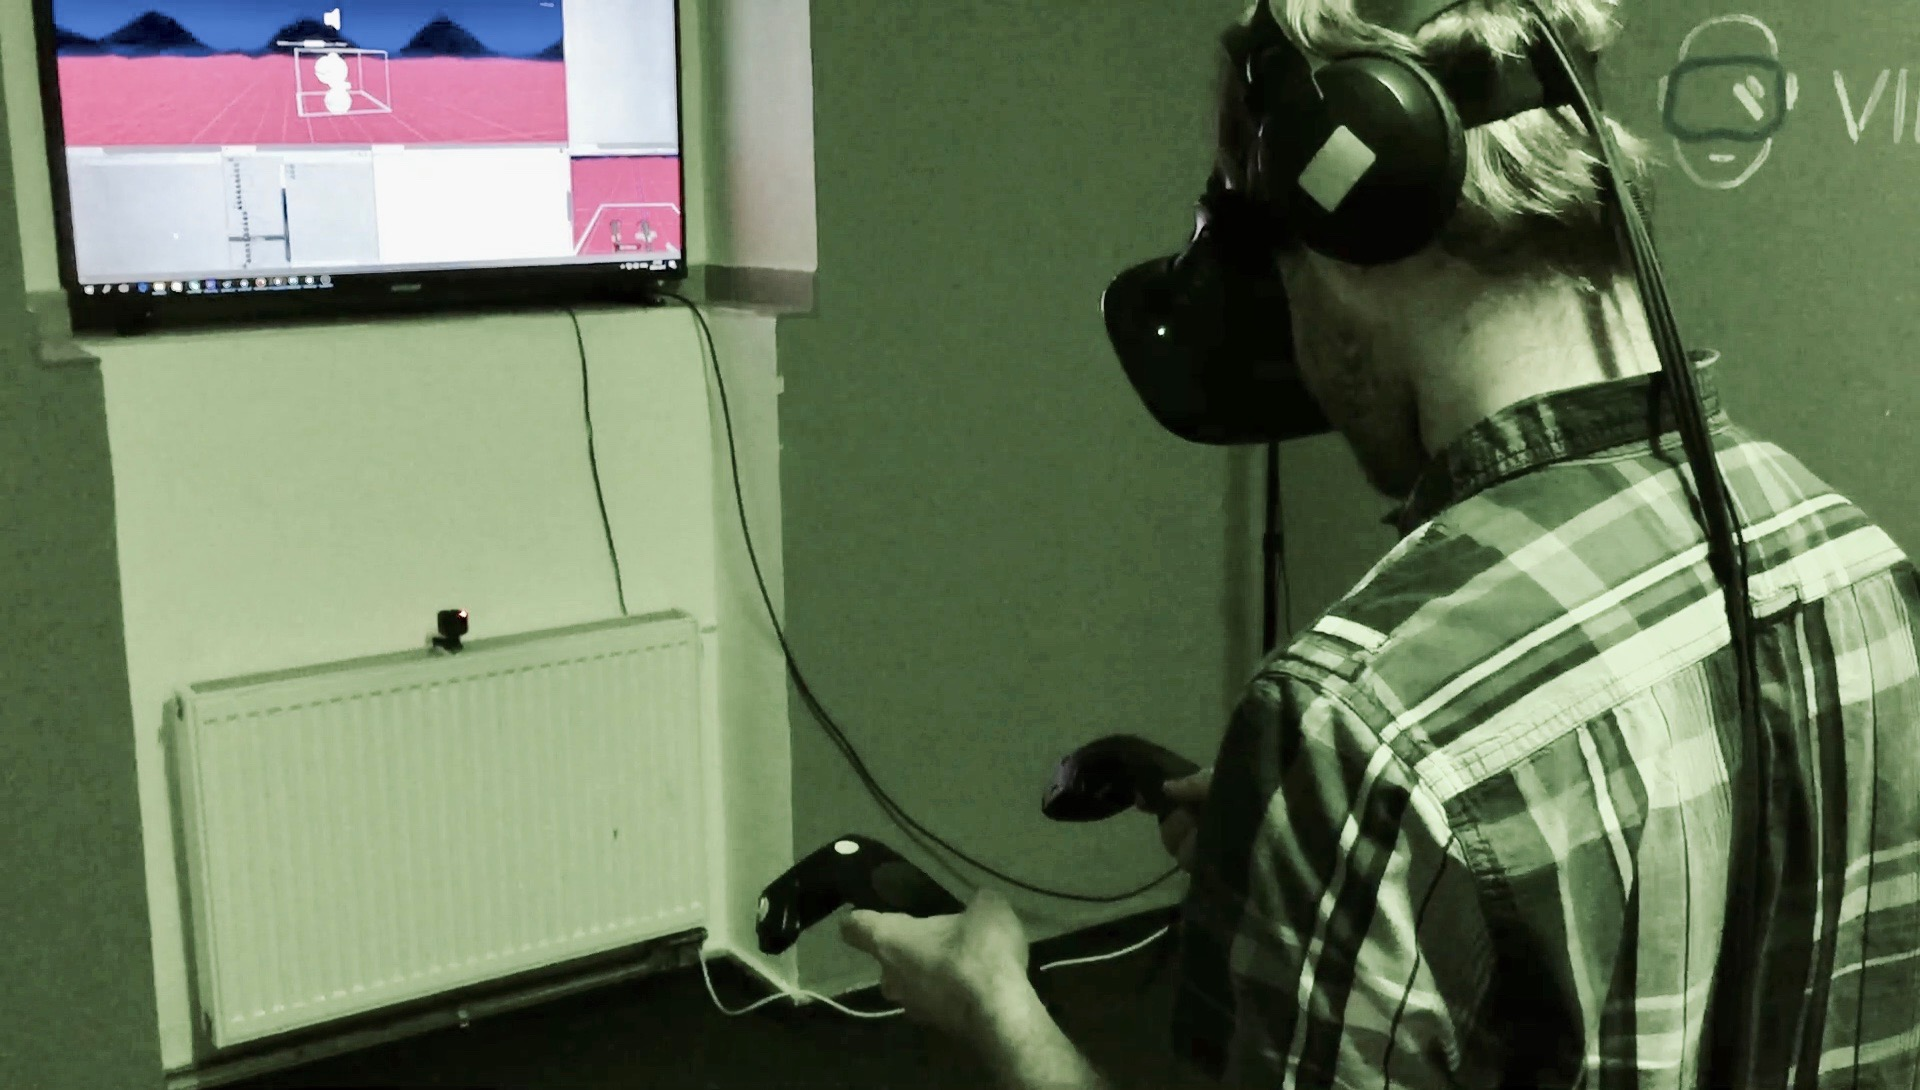
\includegraphics[width=12cm]{src/assets/testing.jpg}
\caption{Fotografie z testování v herně virtuální reality}
\end{figure}

\section{Zjištěné nedostatky a jejich řešení}\label{zjiux161tux11bnuxe9-nedostatky}

Nedostatky v aplikaci jsou převážně technické. Aplikace v době testování trpěla na
chyby v průběhu výuky a vykreslování vizuálního prostředí.

Jako méně závažné lze označit chyby ve vykreslování. Určité prvky rozhraní se v některých
chvílích překrývaly a po skončení výuky byla stále zobrazena nápověda pro stisk
tlačítka, o kterém bylo ve výuce naposledy hovořeno.

Větší problémy představovaly chyby, které přímo ovlivňovaly kvalitu 
výuky. Jednomu z testerů nebylo umožněno stisknout tlačítko na výzvu 
výuky na jednom ze dvou ovladačů. Dalšímu z testerů pak nefungoval 
barevný výběr laserového ukazovátka.

Všechny chyby byly zapsány a budou před produkčním nasazením opraveny.

Testování lze označit jako úspěšné a především užitečné. Odhalilo 
nespočet nedostatků a pozorování chování napomohlo vzniku
několika dalších nápadů, jak aplikaci v budoucnu vylepšit.

\begin{conclusion}
\label{conclusion}
	Cílem této práce bylo vytvořit aplikaci pro usnadnění seznámení s
virtuální realitou návštěvníkům herny a usnandnění obsluhy zaměstnancům
herny.

Byly provedeny analýzy existujících řešení výuky a spouštěčů. Bylo také
pozorováno chování návštěvníků a obsluhy v herně virtuální reality.
Výsledkem analytické části bylo mimo jiné i stanovení funkčních a
nefunkčních požadavků.

Na základě výsledků analýzy pak byla navržena aplikace pro virtuální
realitu skládající se z dvou částí -- z výuky ovládání systému a
spouštěče VR aplikací.

Implementaci navržené aplikace předcházelo ověření korektnosti
navržených funkcionalit principem Proof of Concept, který poukázal na
budoucí komplikace. Jako největší komplikace se ukázalo odchýlení od
rozsahu implementace v podobě nutnosti přidat další komponentu, a to
malý program, tzv. agent, mající na starosti zobrazení spouštěče po
ukončení cizí VR aplikace.

Samotná aplikace byla implementována v jazyce C\# s využitím herního
engine Unity. Součástí implementace bylo zpracování vizuálu, tvorba
prostředí, nadabování průvodce a programování logiky aplikace.

Nakonec byla aplikace otestována v reálném prostředí herny virtuální
reality. Testování dopadlo \ldots{} TODO

\begin{quote}
TODO: obrázek \emph{fig Snímek obrazovky zobrazující kompletní výsledky
celé realizační fáze}
\end{quote}

Realizaci aplikace lze označit za zdárnou. Lze na ní jistě spatřit
následky časové limitace. Velmi omezující byla také nemožnost spouštět
aplikaci na VR systému okamžitě. Vlastní headset je pro studenta
finančně velmi náročná záležitost a tak bylo nutné aplikaci testovat
pouze nárazově způsobem, kdy byla do herny přinesena zkompilovaná
binárka aplikace, otestována, chyby zaznamenány a posléze opraveny.

\section{Možnosti dalšího
vývoje}\label{moux17enosti-dalux161uxedho-vuxfdvoje}

Až v průběhu realizace se naskytly zajímavé možnosti a nápady, jak
aplikaci rozšířit. Bohužel kvůli časovým možnostem nejsou součástí této
závěrečné práce, proto jsou uvedeny v závěru jako příležitosti, jak
aplikaci dále rozšířit a vyvinout.

Knihovna OpenVR je mnohem mocnější, než je na několik prvních pohledů
zjevné. Za vinu to ovšem lze s čistým svědomím klást špatné dokumentaci,
která je nekompletní, nepřehledná a práce s ní není příjemná. Pokud by
se s knihovnou pracovalo na hlubší úrovni a doplnila se dokumentace,
bylo by teoreticky možné vyřešit několik problémů, na které se v práci
narazilo.

Především by mělo být možné nahradit celý \emph{SteamVR Dashboard} a
nedovolit tak zákazníkům přístup k platformě Steam, což by mohlo být pro
herny bezpečnější a systém virtuální reality by tak mohl pracovat v
jakémsi ``kiosk módu''. 

Dále je z nezdokumentovaného kódu zjevné, že v
knihovně existují některé metody pro stahování nainstalovaných VR
aplikací v počítači. Znamenalo by to možnost zobrazit instalované aplikace
nejen z platformy Steam, ale i z platformy Oculus, či Viveport. Pro
účely této závěrečné práce lze však konstatovat, že výsledek nebyl o nic
připraven, jelikož se na platformě Oculus nenacházejí žádné aplikace
určené pro systém HTC Vive a platforma Viveport není v Evropě příliš
populární. Je cílena spíše na asijský trh.

Další zajímavou funkcí by mohlo být jednodušší navázání hry pro více
hráčů. V herně se nacházejí dva systémy HTC Vive a mezi návštěvníky je
oblíbená i hra se spoluhráčem. Také mřížka aplikací by mohla být vylepšena o
doplnění řazení, kupříkladu podle oblíbenosti, určené podle doby, kterou
návštěvníci s aplikací strávili.

Více návrhů na vylepšení aplikace může vzniknout každodenním používáním
v herně po produkčním nasazení.

\end{conclusion}

\printbibliography[title={Zdroje}]

\appendix

\chapter{Seznam použitých zkratek}
\printglossary[type=\acronymtype,style=acronyms]

\chapter{Obsah přiloženého média}

Práce je publikována jako open-source na serveru \emph{GitHub}. Na médiu se nacházejí stažené repozitáře z tohoto serveru. 
Adresáře umístěné v kořenovém adresáři jsou jednotlivé repozitáře a~lze je dohledat i online na následujících adresách:

\begin{itemize}
  \item
    \url{http://github.com/mmajko/bachelors-thesis}
  \item
    \url{http://github.com/mmajko/immersion-vr}
  \item
    \url{http://github.com/mmajko/immersion-vr-agent}
\end{itemize}

\vfill

\begin{dirfigure}%
    \dirtree{%
        .1 bachelor-thesis\DTcomment{projekt textu bakalářské práce}.
            .2 src\DTcomment{další zdrojové soubory}.
            .2 thesis.tex\DTcomment{zdrojový kód textu}.
            .2 thesis.pdf\DTcomment{vygenerovaný text}.
        .1 immersion-vr\DTcomment{projekt aplikace výuky a~spouštěče}.
            .2 Assets\DTcomment{zdroje aplikace}.
            .2 ProjectSettings\DTcomment{nastavení projektu aplikace}.
            .2 bin\DTcomment{zkompilovaný binární program aplikace pro Windows (x64)}.
        .1 immersion-vr-agent\DTcomment{projekt aplikace agenta}.
            .2 Immersion VR~Agent\DTcomment{zdroje aplikace}.
            .2 Immersion VR~Agent.sln\DTcomment{soubor projektu Visual Studio}.
    }
\caption{Obsah přiloženého média}
\end{dirfigure}


\end{document}
